\documentclass[aspectratio=169]{beamer}
\def\thetitle{
  Six Attacks on Matrix
%  \footnote{Full paper available at \url{https://nebuchadnezzar-megolm.github.io/}.}
}
\def\thesubtitle{\url{https://nebuchadnezzar-megolm.github.io/}}
\def\thedate{} % chktex 8
%
% Config
%
\usepackage{chronology}
\usepackage{ulem}
\usepackage{fontawesome}
\usepackage[misc]{ifsym}
\def\courseyear{2022}
\def\thisguy{
Martin Albrecht\\
joint work with Sofía Celi, Benjamin Dowling and Dan Jones}

\def\theemail{}

\title{\Large{\thetitle}}
\subtitle{\thesubtitle}
\author{\thisguy{}}% \href{mailto:\theemail}{\nolinkurl{<\theemail>}}}
\date{\thedate}

\usepackage{amsmath,amsfonts,amssymb,amsthm}
\usepackage{ifxetex,ifluatex}
\usepackage{fixltx2e} % provides \textsubscript
\usepackage{xspace}
\usepackage{graphicx}
\usepackage{booktabs}
\usepackage{comment}
\usepackage{multicol}
\usepackage{url}
\usepackage{relsize}
\usepackage{colortbl}

\renewcommand*{\UrlFont}{\ttfamily\smaller\relax}

%
% Pseudocode
%

\usepackage[linesnumbered,ruled]{algorithm2e}

%
% Source Code Listings
%

\usepackage{listings}
\lstdefinelanguage{Sage}[]{Python}{morekeywords={True,False,sage,cdef,cpdef,ctypedef,self},sensitive=true}
\lstset{frame=none,
          showtabs=False,
          showspaces=False,
          showstringspaces=False,
          commentstyle={\color{mLightBrown}},
          keywordstyle={\color{mLightBrown}\textbf},
          stringstyle ={\color{mDarkBrown}},
          frame=single,
          basicstyle=\tt\smaller\relax,
          backgroundcolor=\color{gray!190!black},
          language = Sage,
          }

%
% Tikz
%

\usepackage{tikz,pgfplots}
\usepackage{tikzpeople}
\usetikzlibrary{calc}
\usetikzlibrary{arrows,automata}
\usetikzlibrary{positioning}
\usetikzlibrary{shapes}
\pgfplotsset{compat=newest}

%% Cache TiKZ pictures

%\usetikzlibrary{external}
%\tikzexternalize[prefix=build/]
%\tikzset{external/up to date check=diff} % MD5 fails from within emacs


%
% Crypto Notation
%

\usepackage[lambda,landau,operators,probability,sets,logic,complexity,asymptotics,adversary]{cryptocode} % after algorithm2e
% always check cryptocode First

\tikzstyle{player} = [rectangle, minimum width=2cm, minimum height=1cm, text centered, draw=black, fill=mLightBrown!50]
\tikzstyle{adversary} = [rectangle, minimum width=2cm, minimum height=1cm, text centered, draw=black, fill=red!50]
% TEXT COMMANDS
\newcommand{\etal}{et~al.\xspace{}}
\newcommand{\ie}{i.e.~}
\newcommand{\eg}{e.g.~}
\newcommand{\ppttxt}{probabilistic polynomial-time}
\mathchardef\mhyphen="2D

%% FIGURE COMMANDS
\definecolor{mBlue}{HTML}{22a1dc}
\definecolor{sBlue}{HTML}{009FE3}
\definecolor{sYellow}{HTML}{FFED00}
\definecolor{sRed}{HTML}{E30613}
\definecolor{sGreen}{HTML}{009640}
\definecolor{sPurple}{HTML}{251B5B}
\definecolor{mGreen}{HTML}{86cd30}
\definecolor{darkgreen}{HTML}{006400}
\definecolor{mLightBrown}{HTML}{e68a00}
\definecolor{lightred}{HTML}{FF9999}

% COLOUR COMMANDS
\newcommand{\sBlue}[1]{\textcolor{sBlue}{#1}}
\newcommand{\sB}[1]{\sBlue{#1}}
\newcommand{\sRed}[1]{\textcolor{sRed}{#1}}
\newcommand{\sR}[1]{\sRed{#1}}
\newcommand{\sGreen}[1]{\textcolor{sGreen}{#1}}
\newcommand{\sG}[1]{\sGreen{#1}}
\newcommand{\sPurple}[1]{\textcolor{Purple}{#1}}
\newcommand{\sP}[1]{\sPurple{#1}}
\newcommand{\sYellow}[1]{\textcolor{sYellow}{#1}}
\newcommand{\sY}[1]{\sYellow{#1}}


% STYLES
\newcommand{\styleAdversary}[1]{\ensuremath{\mathcal{#1}}}
\newcommand{\styleAlgorithm}[1]{\textsf{\upshape #1}}
\newcommand{\styleScheme}[1]{\ensuremath{\mathcal{#1}}}
\newcommand{\styleSecurityNotion}[1]{\ensuremath{\mathsf{#1}}}
\newcommand{\styleQueries}[1]{\ensuremath{\mathsf{#1}}}
\newcommand{\styleVariables}[1]{\ensuremath{\mathit{#1}}}
\newcommand{\styleConstants}[1]{\ensuremath{\mathtt{#1}}}
\newcommand{\styleProtocols}[1]{\ensuremath{\mathtt{#1}}}
\newcommand{\styleOracles}[1]{\ensuremath{\mathrm{#1}}}
\renewcommand{\O}[1]{\ensuremath{\mathsf{#1}}}
\newcommand{\V}[1]{\ensuremath{\mathit{#1}}}

%% FUNCTIONS, SAMPLERS, ETC
\newcommand{\getsr}{\ensuremath{\overset{\$}{\leftarrow}}}
\newcommand{\tor}{\ensuremath{\overset{\$}{\rightarrow}}}
\newcommand{\randcoin}[1]{\ensuremath{\mathcal{R}_{#1}}}
\newcommand{\maxover}[2]{\ensuremath{\underset{#1}{\mathsf{max}}\{#2\}}}
\newcommand{\bits}{\ensuremath{\{0,1\}}}
\newcommand{\rreplace}[1]{\ensuremath{\widetilde{#1}}}

%% GROUPS AND SPACES
\newcommand{\group}{\ensuremath{\mathbb{G}}}
\newcommand{\KeySpace}{\ensuremath{\mathcal{K}}}
\newcommand{\OutputSpace}{\ensuremath{\mathcal{O}}}
\newcommand{\InputSpace}{\ensuremath{\mathcal{I}}}
\newcommand{\NonceSpace}{\ensuremath{\mathcal{N}}}
\newcommand{\MessageSpace}{\ensuremath{\mathcal{M}}}
\newcommand{\HeaderSpace}{\ensuremath{\mathcal{H}}}
\newcommand{\RandomSpace}{\ensuremath{\mathcal{r}}}
\newcommand{\SaltSpace}{\ensuremath{\mathcal{S}}}

%% MATRIX STUFF
\newcommand{\matrixA}{\ensuremath{\mathbf{A}}}
\newcommand{\vectorU}{\ensuremath{\vec{u}}}

 %%DIFFIE-HELLMAN NOTATION
\renewcommand{\secpar}{\ensuremath{\lambda}}
\newcommand{\secparshort}{\ensuremath{k}}
\newcommand{\groupgen}{\ensuremath{\mathcal{G}}}
\newcommand{\generator}{\ensuremath{\V{g}}}

%% ALGORITHMS
\renewcommand{\adversary}{\ensuremath{\mathcal{A}}}
\newcommand{\state}{\ensuremath{st}}
\newcommand{\bdversary}{\ensuremath{\mathcal{B}}}
%\newcommand{\bdv}{\ensuremath{\mathcal{B}}}
\newcommand{\challenger}{\ensuremath{\mathcal{C}}}

%% PROTOCOLS AND ALGORITHMS
\newcommand{\KE}{\ensuremath{\mathsf{KE}}}
\newcommand{\ACCE}{\ensuremath{\mathsf{ACCE}}}
\newcommand{\AKeyGen}{\ensuremath{\mathsf{AKeyGen}}}
\newcommand{\ASKeyGen}{\ensuremath{\mathsf{ASKeyGen}}}
\newcommand{\SKeyGen}{\ensuremath{\mathsf{SKeyGen}}}
\newcommand{\PSKeyGen}{\ensuremath{\mathsf{PSKeyGen}}}
\newcommand{\EKeyGen}{\ensuremath{\mathsf{EKeyGen}}}
\newcommand{\EPKeyGen}{\ensuremath{\mathsf{EPKeyGen}}}
\newcommand{\KeyGen}{\ensuremath{\mathsf{KeyGen}}}
\newcommand{\Muck}{\ensuremath{\mathsf{Muckle}}}

% CRYPTO PRIMITIVES
\newcommand{\DHGen}{\ensuremath{\mathsf{DHGen}}}
\renewcommand{\DH}{\ensuremath{\mathsf{DH}}}
\newcommand{\Hash}{\ensuremath{\mathsf{H}}}
\newcommand{\AEAD}{\ensuremath{\mathsf{AEAD}}}
\newcommand{\Enc}{\ensuremath{\mathsf{Enc}}}
\newcommand{\Dec}{\ensuremath{\mathsf{Dec}}}
\newcommand{\dec}{\ensuremath{\mathsf{Dec}}}
\newcommand{\KDF}{\ensuremath{\mathsf{KDF}}}
\newcommand{\MAC}{\ensuremath{\mathsf{MAC}}}
\newcommand{\Timestamp}{\ensuremath{\mathsf{Timestamp}}}
\newcommand{\PRF}{\ensuremath{\mathsf{PRF}}}
\newcommand{\HKDF}{\ensuremath{\mathsf{HKDF}}}
\newcommand{\KEM}{\ensuremath{\mathsf{KEM}}}
\newcommand{\SIG}{\ensuremath{\mathsf{SIG}}}
\newcommand{\Expand}{\ensuremath{\mathsf{Exp}}}
\newcommand{\Extract}{\ensuremath{\mathsf{Ext}}}
% EXPERIMENT REGISTERS
\newcommand{\Adv}[2]{\ensuremath{\mathsf{Adv}^{#1}_{#2}}}
\newcommand{\Exp}[2]{\ensuremath{\mathsf{Exp}^{#1}_{#2}}}
\newcommand{\protocol}{\ensuremath{\Pi}}
\newcommand{\Dist}{\ensuremath{\mathcal{D}}}
\newcommand{\Prob}{\ensuremath{\mathsf{Pr}}}
\newcommand{\ctr}{\ensuremath{ctr}}
\newcommand{\vecPSK}[1]{\ensuremath{\vec{\mathsf{PSK}_{#1}}}}

% EXPERIMENT PREDICATES
\newcommand{\cleanpredicate}{\ensuremath{\mathsf{clean}}}

% EXPERIMENT CONSTANTS
\newcommand{\numParties}{\ensuremath{n_P}}
\newcommand{\numSessions}{\ensuremath{n_S}}
\newcommand{\numStages}{\ensuremath{n_T}}
\newcommand{\init}{\ensuremath{\styleConstants{init}}}
\newcommand{\resp}{\ensuremath{\styleConstants{resp}}}
\newcommand{\revealflag}{\ensuremath{\styleConstants{revealed}}}
\newcommand{\corruptflag}{\ensuremath{\styleConstants{corrupt}}}
\newcommand{\cleanflag}{\ensuremath{\styleConstants{clean}}}
\newcommand{\inprogress}{\ensuremath{\styleConstants{active}}}
\newcommand{\rejected}{\ensuremath{\styleConstants{reject}}}
\newcommand{\accepted}{\ensuremath{\styleConstants{accept}}}
\newcommand{\trueflag}{\ensuremath{\styleConstants{true}}}
\newcommand{\falseflag}{\ensuremath{\styleConstants{false}}}
%\newcommand{\numX}{\ensuremath{n_X}}

% EXPERIMENT FLAGS
\newcommand{\PSKflag}[1]{\ensuremath{\vec{\mathsf{PSKflag}_{#1}}}}
\newcommand{\SKflag}[1]{\ensuremath{\mathsf{SKflag}_{#1}}}
\newcommand{\ASKflag}[1]{\ensuremath{\mathsf{ASKflag}_{#1}}}
\newcommand{\AKflag}[1]{\ensuremath{\vec{\mathsf{AKflag}_{#1}}}}
\newcommand{\EPKflag}[1]{\ensuremath{\vec{\mathsf{EPKflag}_{#1}}}}
\newcommand{\EKflag}[1]{\ensuremath{\vec{\mathsf{EKflag}_{#1}}}}
\newcommand{\RSKflag}[1]{\ensuremath{\vec{\mathsf{RSKflag}_{#1}}}}
\newcommand{\RKflag}[1]{\ensuremath{\vec{\mathsf{RKflag}_{#1}}}}
\newcommand{\testflag}{\ensuremath{\mathsf{tested}}}

% SESSIONS AND PER-SESSION VARIABLES
\newcommand{\session}{\ensuremath{\pi}}
\newcommand{\sessionid}{\ensuremath{sid}}
\newcommand{\testsess}{\ensuremath{\pi^s_i}}
\newcommand{\partnersess}{\ensuremath{\pi^t_j}}
\newcommand{\partsess}{\ensuremath{\pi^r_j}}
\newcommand{\pk}{\ensuremath{pk}}
\newcommand{\sk}{\ensuremath{sk}}
\newcommand{\psk}{\ensuremath{psk}}
\newcommand{\pskid}{\ensuremath{pskid}}
\newcommand{\status}{\ensuremath{\alpha}}
\newcommand{\pid}{\ensuremath{pid}}
\newcommand{\kid}{\ensuremath{kid}}
\newcommand{\id}{\ensuremath{id}}
\newcommand{\ephkey}{\ensuremath{ek}}
\newcommand{\epubkey}{\ensuremath{epk}}
\renewcommand{\state}{\ensuremath{st}}
\newcommand{\msgsent}{\ensuremath{m_s}}
\newcommand{\msgrecd}{\ensuremath{m_r}}
\newcommand{\role}{\ensuremath{\rho}}

% SECURITY GAME QUERIES
\newcommand{\Test}{\ensuremath{\mathsf{Test}}}
\newcommand{\Corrupt}{\ensuremath{\mathsf{Corrupt}}}
\newcommand{\CorruptASK}{\ensuremath{\mathsf{CorruptASK}}}
\newcommand{\CorruptPK}{\ensuremath{\mathsf{CorruptPK}}}
\newcommand{\CorruptPSK}{\ensuremath{\mathsf{CorruptPSK}}}
\newcommand{\CorruptSK}{\ensuremath{\mathsf{CorruptSK}}}
\newcommand{\CorruptEPK}{\ensuremath{\mathsf{CorruptEPK}}}
\newcommand{\CorruptEK}{\ensuremath{\mathsf{CorruptEK}}}
\newcommand{\RevealRandom}{\ensuremath{\mathsf{RevealRandom}}}
\newcommand{\Reveal}{\ensuremath{\mathsf{Reveal}}}
\newcommand{\Create}{\ensuremath{\mathsf{Create}}}
\newcommand{\CreatePSK}{\ensuremath{\mathsf{CreatePSK}}}
\newcommand{\Send}{\ensuremath{\mathsf{Send}}}
\newcommand{\CompromiseQK}{\ensuremath{\mathsf{CompromiseQK}}}
\newcommand{\CompromiseSK}{\ensuremath{\mathsf{CompromiseSK}}}
\newcommand{\CompromiseSS}{\ensuremath{\mathsf{CompromiseSS}}}



%% SECURITY GAME NOTIONS
\newcommand{\COLL}{\styleSecurityNotion{coll}}
\newcommand{\coll}{\styleSecurityNotion{coll}}
\newcommand{\ddh}{\styleSecurityNotion{ddh}}
\newcommand{\dualkdf}{\styleSecurityNotion{dual}\mhyphen \styleSecurityNotion{kdf}}
\newcommand{\dualprf}{\styleSecurityNotion{dual}\mhyphen \styleSecurityNotion{prf}}
\newcommand{\prf}{\styleSecurityNotion{prf}}
\newcommand{\aead}{\styleSecurityNotion{aead}}
\newcommand{\auth}{\styleSecurityNotion{auth}}
\newcommand{\kdf}{\styleSecurityNotion{kdf}}
\newcommand{\PRFODH}{\ensuremath{\mathsf{PRFODH}}}
\newcommand{\eCKPFS}{\ensuremath{\mathsf{eCK}\mhyphen \mathsf{PFS}}}
\newcommand{\eCKPFSPSK}{\ensuremath{\mathsf{eCK}\mhyphen \mathsf{PFS} \mhyphen \mathsf{PSK}}}
\newcommand{\symlrPRFODH}{\ensuremath{\mathsf{sym}\mhyphen\mathsf{lr}\mhyphen \PRFODH}}
\newcommand{\lrPRFODH}{\ensuremath{\mathsf{lr}\mhyphen \PRFODH}}
\newcommand{\snPRFODH}{\ensuremath{\mathsf{sn}\mhyphen \PRFODH}}
\newcommand{\dualsnPRFODH}{\ensuremath{\mathsf{d}\mhyphen\mathsf{sn}\mhyphen \PRFODH}}
\newcommand{\ssPRFODH}{\ensuremath{\mathsf{ss}\mhyphen \PRFODH}}
\newcommand{\mnPRFODH}{\ensuremath{\mathsf{mn}\mhyphen \PRFODH}}
\newcommand{\msPRFODH}{\ensuremath{\mathsf{ms}\mhyphen \PRFODH}}
\newcommand{\mmPRFODH}{\ensuremath{\mathsf{mm}\mhyphen \PRFODH}}
\newcommand{\symsnPRFODH}{\ensuremath{\mathsf{sym}\mhyphen\mathsf{sn}\mhyphen \PRFODH}}
\newcommand{\symssPRFODH}{\ensuremath{\mathsf{sym}\mhyphen\mathsf{ss}\mhyphen \PRFODH}}
\newcommand{\symmsPRFODH}{\ensuremath{\mathsf{sym}\mhyphen\mathsf{ms}\mhyphen \PRFODH}}
\newcommand{\symmmPRFODH}{\ensuremath{\mathsf{sym}\mhyphen\mathsf{mm}\mhyphen \PRFODH}}
\newcommand{\symmnPRFODH}{\ensuremath{\mathsf{sym}\mhyphen\mathsf{mn}\mhyphen \PRFODH}}
%\newcommand{\ODH}{\ensuremath{\mathsf{ODH}}}
\newcommand{\eufqcma}{\ensuremath{\mathsf{q}\mhyphen\mathsf{euf}\mhyphen\mathsf{cma}}}
\newcommand{\EUFCMA}{\ensuremath{\mathsf{EUF}\mhyphen\mathsf{CMA}}}
\newcommand{\OTKEX}{\ensuremath{\mathsf{HAKE}}}
\newcommand{\indcpa}{\ensuremath{\mathsf{ind}\mhyphen\mathsf{cpa}}}

% COMMENTS
\newcommand{\ben}[1]{\textcolor{purple}{bd: #1}}
\newcommand{\kenny}[1]{\textcolor{red}{kgp: #1}}
\newcommand{\examplecomment}[1]{\textcolor{blue}{ex: #1}}

% WIREGUARD VARIABLES
\newcommand{\seed}{\ensuremath{C}}
\newcommand{\hash}{\ensuremath{H}}
\newcommand{\ID}[1]{\ensuremath{ID_{#1}}}
\newcommand{\wg}{\ensuremath{\mathsf{WG}}}
\newcommand{\mwg}{\ensuremath{\mathsf{mWG}}}
\newcommand{\wkey}{\ensuremath{\kappa}}
\newcommand{\PSK}{\ensuremath{psk}}
\newcommand{\now}{\ensuremath{now}}
\newcommand{\cookie}{\ensuremath{cookie}}
\newcommand{\tk}[1]{\ensuremath{tk_{#1}}}

% WIREGUARD MESSAGES AND FIELDS
\newcommand{\SendHello}{\ensuremath{\mathtt{InitiatorHello}}}  %% changed from send to initiator for consistency with WG paper
\newcommand{\sSendHello}{\ensuremath{\mathtt{InitHello}}}
\newcommand{\ssSendHello}{\ensuremath{\mathtt{SH}}}
\newcommand{\RespHello}{\ensuremath{\mathtt{ResponderHello}}}
\newcommand{\sRespHello}{\ensuremath{\mathtt{RespHello}}}
\newcommand{\ssRespHello}{\ensuremath{\mathtt{RH}}}
\newcommand{\lbl}[1]{\ensuremath{\mathtt{label}_{#1}}}
\newcommand{\type}{\ensuremath{\mathtt{type}}}
\newcommand{\etk}{\ensuremath{\mathtt{etk}}}
\newcommand{\epk}{\ensuremath{\mathtt{epk}}}
\newcommand{\ltk}{\ensuremath{\mathtt{ltk}}}
\newcommand{\sid}[1]{\ensuremath{\mathtt{sid}_{#1}}}
\newcommand{\tstamp}{\ensuremath{\mathtt{time}}}
\newcommand{\firstmac}{\ensuremath{\mathtt{mac1}}}
\newcommand{\secondmac}{\ensuremath{\mathtt{mac2}}}
\newcommand{\zero}{\ensuremath{\mathtt{zero}}}

% Notation


% Math
\newcommand{\probnot}[1]{\overline{#1}}
\newcommand{\bitsnum}[2]{{\ll \hspace{-0.25em} \mathbf{#1} \hspace{-0.25em} \gg}_{#2}}
\newcommand{\bitspace}[1]{\ensuremath{\{0,1\}^{#1}}}
\renewcommand{\concat}{\ensuremath{\mathbin{\|}}}
\mathchardef\mhyphen="2D

\newcommand{\assign}{\leftarrow}
\newcommand{\evaluatesto}{\Rightarrow}

\newcommand{\pairwisedistinct}{\pcalgostyle{PairwiseDistinct}}
\newcommand{\collision}{\pcalgostyle{Coll}}
\newcommand{\nocollision}{\pcalgostyle{NoColl}}



% Secure Pairwise Channels: Signal & Olm
\newcommand{\SecureChannel}{\pcalgostyle{SC}}
\newcommand{\SecureChannelKGen}{\SecureChannel.\pcalgostyle{KGen}}
\newcommand{\SecureChannelIKE}{\SecureChannel.\pcalgostyle{IKE}}
\newcommand{\SecureChannelEnc}{\SecureChannel.\pcalgostyle{Enc}}
\newcommand{\SecureChannelDec}{\SecureChannel.\pcalgostyle{Dec}}

\newcommand{\Signal}{\pcalgostyle{Signal}}
\newcommand{\SignalKGen}{\Signal.\pcalgostyle{KGen}}
\newcommand{\SignalIKE}{\Signal.\pcalgostyle{IKE}}
\newcommand{\SignalEnc}{\Signal.\pcalgostyle{Enc}}
\newcommand{\SignalDec}{\Signal.\pcalgostyle{Dec}}

\newcommand{\Olm}{\pcalgostyle{Olm}}
\newcommand{\OlmKGen}{\Olm.\pcalgostyle{KGen}}
\newcommand{\OlmIKE}{\Olm.\pcalgostyle{IKE}}
\newcommand{\OlmEnc}{\Olm.\pcalgostyle{Enc}}
\newcommand{\OlmDec}{\Olm.\pcalgostyle{Dec}}
\newcommand{\OlmCmp}{\Olm.\pcalgostyle{Cmp}}
\newcommand{\OlmAlgorithmString}{\ensuremath{\mathtt{m.olm.v1.curve25519-aes-sha2}}}
\newcommand{\OlmState}[1][]{\ifthenelse{\equal{#1}{}}{\pi_{\pcvar{olm}}}{\pi_{\pcvar{olm},#1}}}
\newcommand{\OlmStates}[1][]{\ifthenelse{\equal{#1}{}}{\Pi_{\pcvar{olm}}}{\Pi_{\pcvar{olm},#1}}}

\newcommand{\OlmIdentitySK}[1][]{\ifthenelse{\equal{#1}{}}{isk}{isk_{#1}}}
\newcommand{\OlmIdentityPK}[1][]{\ifthenelse{\equal{#1}{}}{ipk}{ipk_{#1}}}
\newcommand{\OlmEphemSK}[1][]{\ifthenelse{\equal{#1}{}}{esk}{esk_{#1}}}
\newcommand{\OlmEphemPK}[1][]{\ifthenelse{\equal{#1}{}}{epk}{epk_{#1}}}


% Megolm

\newcommand{\Megolm}{\pcalgostyle{Megolm}}
\newcommand{\MegolmReg}{\Megolm.\pcalgostyle{Register}}
\newcommand{\MegolmInit}{\Megolm.\pcalgostyle{Init}}
\newcommand{\MegolmAddDevice}{\Megolm.\pcalgostyle{Add}}
\newcommand{\MegolmRemoveDevice}{\Megolm.\pcalgostyle{Remove}}
\newcommand{\MegolmEnc}{\Megolm.\pcalgostyle{Encrypt}}
\newcommand{\MegolmDec}{\Megolm.\pcalgostyle{Decrypt}}
\newcommand{\MegolmAdv}{\Megolm.\pcalgostyle{Advance}}
\newcommand{\MegolmAlgorithmString}{\ensuremath{\mathtt{m.megolm.v1.aes-sha2}}}
\newcommand{\MegolmSignature}{\ensuremath{\sigma_{\pcvar{mg}}}}
\newcommand{\MegolmVersion}{\ensuremath{\pcvar{ver}}}
\newcommand{\MegolmState}[1][]{\ifthenelse{\equal{#1}{}}{\pi_{\pcvar{mg}}}{\pi_{\pcvar{mg},#1}}}
\newcommand{\MegolmStates}[1][]{\ifthenelse{\equal{#1}{}}{\Pi_{\pcvar{mg}}}{\Pi_{\pcvar{mg},#1}}}

\newcommand{\MegolmRatchet}{\pcalgostyle{MegolmRatchet}}
\newcommand{\MegolmRatchetInit}{\MegolmRatchet.\pcalgostyle{Init}}
\newcommand{\MegolmRatchetNext}{\MegolmRatchet.\pcalgostyle{Next}}
\newcommand{\MegolmRatchetAdv}{\MegolmRatchet.\pcalgostyle{Advance}}

\newcommand{\ratchetkdf}{\pcalgostyle{RatchetKDF}}
\newcommand{\ratchetkdfinit}{\ratchetkdf.\pcalgostyle{Init}}
\newcommand{\ratchetkdfnext}{\ratchetkdf.\pcalgostyle{Next}}

\newcommand{\ratchetgamenext}{\pcalgostyle{Next}}
\newcommand{\ratchetgamecomp}{\pcalgostyle{Compromise}}
\newcommand{\ratchetgamecompromise}{\ratchetgamecomp}

\newcommand{\MegolmKeysConst}{\mathtt{``MEGOLM\_KEYS"}}

\newcommand{\hhc}[2]{(#1, #2)\mathsf{-hierarchical\ hash\ chain}}

\newcommand{\jsonencode}{\pcalgostyle{JSON.Encode}}
\newcommand{\jsondecode}{\pcalgostyle{JSON.Decode}}

\newcommand{\MegolmPK}[1][]{\ifthenelse{\equal{#1}{}}{gpk}{gpk_{#1}}}
\newcommand{\MegolmSK}[1][]{\ifthenelse{\equal{#1}{}}{gsk}{gsk_{#1}}}
\newcommand{\MegolmIS}{\ensuremath{\mathfrak{S}_{\MegolmPK[]}}}
\newcommand{\MegolmOS}{\ensuremath{\mathfrak{S}_{\MegolmSK[]}}}

% Cross Signing / Verification Framework

\newcommand{\CrossSign}{\pcalgostyle{CrossSign}}
\newcommand{\CrossSignInit}{\CrossSign.\pcalgostyle{Init}}
\newcommand{\CrossSignSignUser}{\CrossSign.\pcalgostyle{SignUser}}
\newcommand{\CrossSignSignDevice}{\CrossSign.\pcalgostyle{SignDevice}}
\newcommand{\CrossSignVerifyDevice}{\CrossSign.\pcalgostyle{VerifyDevice}}
\newcommand{\CrossSignKeyUsage}{\mathsf{usage}}
\newcommand{\CrossSignConstantMaster}{\mathtt{master}}
\newcommand{\CrossSignConstantSelfSign}{\mathtt{self\_signing}}
\newcommand{\CrossSignConstantUserSign}{\mathtt{user\_signing}}
\newcommand{\CrossSignState}[1][]{\ifthenelse{\equal{#1}{}}{\pi_{\pcvar{cs}}}{\pi_{\pcvar{cs},#1}}}
\newcommand{\CrossSignUserKeyPackage}[1]{u_{#1}}
\newcommand{\CrossSignDeviceRegistration}{\rho_{\pcvar{reg}}}
\newcommand{\CrossSignUserTrust}{\rho_{\pcvar{trust}}}
\newcommand{\MasterSK}[1][]{\ifthenelse{\equal{#1}{}}{msk}{msk_{#1}}}
\newcommand{\MasterPK}[1][]{\ifthenelse{\equal{#1}{}}{mpk}{mpk_{#1}}}
\newcommand{\UserSK}[1][]{\ifthenelse{\equal{#1}{}}{usk}{usk_{#1}}}
\newcommand{\UserPK}[1][]{\ifthenelse{\equal{#1}{}}{upk}{upk_{#1}}}
\newcommand{\SelfSK}[1][]{\ifthenelse{\equal{#1}{}}{ssk}{ssk_{#1}}}
\newcommand{\SelfPK}[1][]{\ifthenelse{\equal{#1}{}}{spk}{spk_{#1}}}

\newcommand{\CrossSignStateUnpack}
{(d, u, t, \MasterSK, \UserSK, \SelfSK) \assign \CrossSignState}
\newcommand{\CrossSignStatePack}
{\CrossSignState \assign (d, u, t, \MasterSK, \UserSK, \SelfSK)}


% SAS

\newcommand{\SAS}{\ensuremath{\pcalgostyle{SAS}}\xspace}
\newcommand{\SASCalculateMAC}{\ensuremath{\SAS.\pcalgostyle{CalcMAC}}\xspace}
\newcommand{\SASSendMAC}{\ensuremath{\SAS.\pcalgostyle{SendMAC}}\xspace}
\newcommand{\SASVerifyMAC}{\ensuremath{\SAS.\pcalgostyle{VerifyMAC}}\xspace}
\newcommand{\SASSignMAC}{\ensuremath{\SAS.\pcalgostyle{SignDevice}}\xspace}

\newcommand{\MsgTypeVerificationMAC}{%
	\ifmmode \mathtt{m.key.verification.mac}\xspace%
	\else \texttt{m.key.verification.mac}\xspace%
	\fi%
}


% Key Sharing

\newcommand{\KeyShare}{\pcalgostyle{KeyShare}}
\newcommand{\KeyShareRequest}{\KeyShare.\pcalgostyle{Request}}
\newcommand{\KeyShareShare}{\KeyShare.\pcalgostyle{Share}}
\newcommand{\KeyShareRecover}{\KeyShare.\pcalgostyle{Recover}}


% Secrets Module

\newcommand{\MsgTypeSecretsRequest}{%
	\ifmmode \mathtt{m.secret.requests}\xspace%
	\else \texttt{m.secret.requests}\xspace%
	\fi%
}

\newcommand{\MsgTypeSecretsSend}{%
	\ifmmode \mathtt{m.secret.send}\xspace%
	\else \texttt{m.secret.send}\xspace%
	\fi%
}


% Matrix Messaging

\newcommand{\Matrix}{\ensuremath{\pcalgostyle{Matrix}}}
\newcommand{\MatrixGen}{\ensuremath{\Matrix.\pcalgostyle{Gen}}}
\newcommand{\MatrixReg}{\ensuremath{\Matrix.\pcalgostyle{Reg}}}
\newcommand{\MatrixInit}{\ensuremath{\Matrix.\pcalgostyle{Init}}}
\newcommand{\MatrixRecv}{\ensuremath{\Matrix.\pcalgostyle{Recv}}}
\newcommand{\MatrixExec}{\ensuremath{\Matrix.\pcalgostyle{Exec}}}
\newcommand{\MatrixAdd}{\ensuremath{\Matrix.\pcalgostyle{Add}}}
\newcommand{\MatrixRemove}{\ensuremath{\Matrix.\pcalgostyle{Remove}}}
\newcommand{\MatrixEncrypt}{\ensuremath{\Matrix.\pcalgostyle{Encrypt}}}
\newcommand{\MatrixDecrypt}{\ensuremath{\Matrix.\pcalgostyle{Decrypt}}}
\newcommand{\MatrixKeyRequest}{\ensuremath{\Matrix.\pcalgostyle{KeyRequest}}}
\newcommand{\MatrixKeyShare}{\ensuremath{\Matrix.\pcalgostyle{KeyShare}}}
\newcommand{\MatrixKeyRecover}{\ensuremath{\Matrix.\pcalgostyle{KeyRecover}}}
\newcommand{\MatrixState}{\ensuremath{\pi_{\pcvar{mt}}}}

\newcommand{\DeviceKeyPackage}{m_{\pcvar{dev}}}  % A self-signed package for the device identity
\newcommand{\Algorithm}{\pcvar{alg}}
\newcommand{\DeviceMapping}[1][]{\ifthenelse{\equal{#1}{}}{\pcvar{DM}}{\pcvar{DM}_{#1}}}

\newcommand{\MsgTypeEncrypted}{%
	\ifmmode \mathtt{m.room.encrypted}\xspace%
	\else \texttt{m.room.encrypted}\xspace%
	\fi%
}
\newcommand{\MsgTypeMessage}{%
	\ifmmode \mathtt{m.room.message}\xspace%
	\else \texttt{m.room.message}\xspace%
	\fi%
}
\newcommand{\MsgTypeRoomKey}{%
	\ifmmode \mathtt{m.room\_key}\xspace%
	\else \texttt{m.room\_key}\xspace%
	\fi%
}
\newcommand{\MsgTypeRoomKeyRequest}{%
	\ifmmode \mathtt{m.room\_key\_request}\xspace%
	\else \texttt{m.room\_key\_request}\xspace%
	\fi%
}
\newcommand{\MsgTypeFwdRoomKey}{%
	\ifmmode \mathtt{m.forwarded\_room\_key}\xspace%
	\else \texttt{m.forwarded\_room\_key}\xspace%
	\fi%
}

\newcommand{\DeviceSK}[1][]{\ifthenelse{\equal{#1}{}}{dsk}{dsk_{#1}}}
\newcommand{\DevicePK}[1][]{\ifthenelse{\equal{#1}{}}{dpk}{dpk_{#1}}}

\newcommand{\MatrixStateUnpack}
{(U, D, G, \role, \DeviceMapping, \CrossSignState, \MegolmStates, \OlmStates, T) \assign \MatrixState}
\newcommand{\MatrixStatePack}
{\MatrixState \assign (U, D, G, \role, \DeviceMapping, \CrossSignState, \MegolmStates, \OlmStates, T)}

% Homeserver

\newcommand{\HS}{\pcalgostyle{HS}}
\newcommand{\HSGetDevicePK}{\HS.\pcalgostyle{GetDevicePK}}
\newcommand{\HSGetDeviceKeys}{\HS.\pcalgostyle{GetDeviceKeys}}
\newcommand{\HSGetCrossSigningMasterPK}{\HS.\pcalgostyle{GetCrossSigningMasterPK}}



% Ciphertext types
%
% Encrypted messages in Matrix can be wrapped in a few layers. Usually:
%   1. Actual message
%   2. (1) wrapped with event metadata like the event type (e.g. m.room_key), room_id etc.
%   3. Encryption of (2) by Olm or Megolm
%   4. Unauthenticated, plaintext wrapper of (3). This is the m.room.encrypted message.
%
% I had been using inconsistent notation to refer to these and it was all a bit confusing.
% Let's standardise it with the commands below:

\newcommand{\MsgPlaintext}{m}
\newcommand{\MsgCiphertext}{c}


% Crypto Primitives

\DeclareMathOperator{\hkdf}{\mathsf{HKDF}}
\DeclareMathOperator{\hmac}{\mathsf{HMAC}}
\DeclareMathOperator{\sha256}{\mathsf{SHA-256}}
\DeclareMathOperator{\hkdfsha256}{\mathsf{HKDF\mhyphen SHA\mhyphen 256}}
\DeclareMathOperator{\hmacsha256}{\mathsf{HMAC\mhyphen SHA\mhyphen 256}}
\DeclareMathOperator{\aescbc}{\mathsf{AES}\mhyphen\mathsf{CBC}}

\newcommand{\XDH}{\pcalgostyle{X25519}}
\newcommand{\XDHKGen}{\XDH.\kgen}
\newcommand{\XDHSklen}{{\XDH.\pcalgostyle{skl}}}
\newcommand{\XDHPklen}{{\XDH.\pcalgostyle{pkl}}}

\newcommand{\ed}{\pcalgostyle{Ed25519}}
\newcommand{\edkgen}{\ed.\kgen}
\newcommand{\edsign}{\ed.\pcalgostyle{Sign}}
\newcommand{\edverify}{\ed.\pcalgostyle{Verify}}
\newcommand{\edsklen}{{\ed.\pcalgostyle{skl}}}
\newcommand{\edpklen}{{\ed.\pcalgostyle{pkl}}}

\newcommand{\ds}{\pcalgostyle{DS}}
\newcommand{\dskgen}{{\ds.\kgen}}
\newcommand{\dssign}{{\ds.\pcalgostyle{Sign}}}
\newcommand{\dsverify}{\ds.\pcalgostyle{Verify}}
\newcommand{\dssklen}{{\ds.\pcalgostyle{skl}}}
\newcommand{\dspklen}{{\ds.\pcalgostyle{pkl}}}

\newcommand{\se}{\pcalgostyle{SE}}
\newcommand{\seenc}{{\se.\enc}}
\newcommand{\sedec}{{\se.\dec}}

\newcommand{\ff}{\pcalgostyle{F}}
\newcommand{\iv}{\pckeystyle{iv}}
\newcommand{\pcvar}[1]{\mathsf{#1}}

\newcommand{\UGKE}{\pcalgostyle{UGKE}}
\newcommand{\PUGKE}{\pcalgostyle{PUGKE}}
\newcommand{\DOGM}{\ensuremath{\mathbf{DOGM}}}
\newcommand{\Reg}{\mathbf{Reg}}
\newcommand{\Add}{\mathbf{Add}}
\newcommand{\Remove}{\mathbf{Remove}}
\newcommand{\Encrypt}{\mathbf{Encrypt}}
\newcommand{\Decrypt}{\mathbf{Decrypt}}
\newcommand{\Gen}{\mathbf{Gen}}
\newcommand{\Exec}{\pcalgostyle{Exec}}
\newcommand{\Init}{\mathbf{Init}}
\newcommand{\Proc}{\pcalgostyle{Proc}}
\newcommand{\ProcAdd}{\pcalgostyle{ProcessAdd}}
\newcommand{\ProcRemove}{\pcalgostyle{ProcessRemove}}
\newcommand{\StateRecv}{\pcalgostyle{StateRecv}}
\newcommand{\StateShare}{\pcalgostyle{StateShare}}
\newcommand{\StateReq}{\pcalgostyle{StateReq}}

%% PROTOCOL INTERFACES
\newcommand{\mem}{\pcalgostyle{mem}}
\newcommand{\rec}{\pcalgostyle{rec}}
\newcommand{\pau}{\pcalgostyle{pau}}


% ALGORITHMS
\renewcommand{\adversary}{\ensuremath{\mathcal{A}}}

%% SPACES
\newcommand{\pauspace}{\ensuremath{\mathcal{P}_{k}}}
\newcommand{\sauspace}{\ensuremath{\mathcal{S}_{k}}}
\newcommand{\psspace}{\ensuremath{\mathcal{PSS}}}
\newcommand{\sstate}{\ensuremath{\mathcal{ST}}}
\newcommand{\iid}{\ensuremath{\mathcal{IID}}}

\newcommand{\kidpace}{\ensuremath{\mathcal{K}_{id}}}
\newcommand{\gidspace}{\ensuremath{\mathcal{G}_{id}}}
\newcommand{\didspace}{\ensuremath{\mathcal{D}_{id}}}
\newcommand{\uidspace}{\ensuremath{\mathcal{U}_{id}}}

\newcommand{\uid}{\ensuremath{A}}
\newcommand{\did}{\ensuremath{i}}
\newcommand{\gid}{\ensuremath{G}}

\newcommand{\cmd}{\ensuremath{\mathcal{CMD}}}
\newcommand{\ctxt}{\ensuremath{\mathcal{C}}}
\newcommand{\keyspace}{\ensuremath{\mathcal{K}}}
\newcommand{\sidspace}{\ensuremath{\mathcal{SID}}}
\newcommand{\msgspace}{\ensuremath{\mathcal{M}}}

% EXPERIMENT CONSTANTS
\newcommand{\numComm}{\ensuremath{n_C}}
\newcommand{\numDevice}{\ensuremath{n_D}}
\newcommand{\numGroups}{\ensuremath{n_G}}
\newcommand{\numMsg}{\ensuremath{n_M}}
\newcommand{\send}{\ensuremath{\styleConstants{send}}}
\newcommand{\recv}{\ensuremath{\styleConstants{recv}}}
%\newcommand{\numX}{\ensuremath{n_X}}

% EXPERIMENT FLAGS
\newcommand{\DKflag}[2]{\ensuremath{\mathsf{DKflag}_{#1}^{#2}}}
\newcommand{\GSflag}[2]{\ensuremath{\mathsf{GSflag}_{#1}^{#2}}}
\newcommand{\USflag}[1]{\ensuremath{\mathtt{UsS}_{#1}}}
\newcommand{\DSflag}[1]{\ensuremath{\mathtt{DeS}_{#1}}}
\newcommand{\SSflag}[1]{\ensuremath{\mathtt{SeS}_{#1}}}

% SESSIONS AND PER-SESSION VARIABLES
\renewcommand{\state}{\ensuremath{st}}
\newcommand{\clean}{\ensuremath{clean}}

% SECURITY GAME QUERIES
\newcommand{\CorruptUser}{\ensuremath{\mathsf{CorruptUser}}}
\newcommand{\CorruptDevice}{\ensuremath{\mathsf{CorruptDevice}}}
\newcommand{\Compromise}{\ensuremath{\mathsf{Compromise}}}
\newcommand{\AddMember}{\ensuremath{\mathsf{AddMember}}}
\newcommand{\RemoveMember}{\ensuremath{\mathsf{RemoveMember}}}
\newcommand{\Chall}{\mathsf{Challenge}}



% SECURITY GAME NOTIONS
\newcommand{\PFSUGKE}{\ensuremath{\mathsf{PFS}\mhyphen \mathsf{UGKE}}}
\newcommand{\KIND}{\ensuremath{\mathsf{KIND}}}


% Crypto Games

\newcommand{\game}[2]{\pcalgostyle{Game}^{\mathcal{#1}}_{\pcalgostyle{#2}}}


% Security Definitions

\newcommand{\rkdfsecure}[3]{(#1, #2, #3)\textsf{-secure ratcheted key derivation function}}


% Actors/variable scoping

\definecolor{scopeprivate}{RGB}{255,99,71}
\definecolor{scopeinsider}{RGB}{0,205,00}
\definecolor{scopeoutsider}{RGB}{58,95,255}

\newcommand{\scopeprivate}[1]{\textcolor{scopeprivate}{#1}}
\newcommand{\scopeinsider}[1]{\textcolor{scopeinsider}{#1}}
\newcommand{\scopeoutsider}[1]{\textcolor{scopeoutsider}{#1}}

\newcommand{\sessionout}{S^{\mathsf{OUT}}}
\newcommand{\sessionin}{S^{\mathsf{IN}}}

% Keys
\newcommand{\fingerprintkey}{\pckeystyle{fk}}
\newcommand{\olmkeys}{\pckeystyle{ok}}


% Pseudocode
\newcommand{\pcbreak}{\highlightkeyword{break}}



%
% Metropolis Theme
% https://github.com/matze/mtheme.git
%

\usetheme{metropolis}

%
% UTF-8 all the things
% 
%\usepackage{unicodesymbols} % put this after m which loads fontspec


%
% BibLaTeX
%

\usepackage[
    backend=bibtex,
]{biblatex}

\addbibresource{local.bib}
\addbibresource{cryptobib/abbrev3.bib}
\addbibresource{cryptobib/crypto_crossref.bib}

\DeclareFieldFormat{title}{\alert{#1}}
\DeclareFieldFormat[book]{title}{\alert{#1}}
\DeclareFieldFormat[inproceedings]{title}{\alert{#1}}
\DeclareFieldFormat[article]{title}{\alert{#1}}
\DeclareFieldFormat[misc]{title}{\alert{#1}}

%
% Microtype
%

\IfFileExists{upquote.sty}{\usepackage{upquote}}{}
\IfFileExists{microtype.sty}{\usepackage{microtype}}{}


\setlength{\parindent}{0pt}
\setlength{\parskip}{6pt plus 2pt minus 1pt}
\setlength{\emergencystretch}{3em}  % prevent overfull lines
\setcounter{secnumdepth}{0}


\AtBeginSection[] % Do nothing for \section*
{
\begin{frame}<beamer>
\frametitle{Outline}
\tableofcontents[currentsection]
\end{frame}
}

%
% Metadata, give the NSA something to collect which totally doesn't invade our privacy
%

\hypersetup{pdfauthor={\thisguy},
            pdfsubject={\thesubtitle}}

%
% Handouts
%

\ifdefined\ishandout
\usepackage{pgfpages}
\pgfpagesuselayout{4 on 1}[a4paper,border shrink=5mm,landscape]
\fi



\usepackage[export]{adjustbox}
% FIGURE COMMANDS
\definecolor{mBlue}{HTML}{22a1dc}
\definecolor{mGreen}{HTML}{86cd30}
\definecolor{darkgreen}{HTML}{006400}
\definecolor{mLightBrown}{HTML}{e68a00}

%% MATH MODE COLOR BOXES
\newcommand{\highlight}[2][yellow]{\mathchoice%
	{\colorbox{#1}{$\displaystyle#2$}}%
	{\colorbox{#1}{$\textstyle#2$}}%
	{\colorbox{#1}{$\scriptstyle#2$}}%
	{\colorbox{#1}{$\scriptscriptstyle#2$}}}%

% ClientAction and ServerAction
% Print a command executed by the client/server
% 1st argument: the text
\newcommand{\ClientAction}[1]{
	\node[right] at (\InitX, \Y) {#1};
}
\newcommand{\ServerAction}[1]{
	\node[left] at (\RespX, \Y) {#1};
}
\newcommand{\SharedAction}[1]{
	\node at ($1/2*(\InitX, \Y)+1/2*(\RespX, \Y)$) {#1};
}
\newcommand{\AdversaryAction}[1]{
	\node at ($1/2*(\InitX, \Y)+1/2*(\RespX, \Y)$) {\textcolor{red}{#1}};
}
% ClientToServer and ServerToClient
% Draws a message flow from client-to-server or server-to-client, with text above and below
% 1st argument (optional): line type, default ->
% 2nd argument: text above
% 3rd argument: text below
% Example: \ClientToServer{$Y$}{}
% Example: \ClientToServer[<->,double]{$Y$}{over an encrypted channel}
\newcommand{\ClientToServer}[3][->]{
	\NextLine[0.5]
	\draw[#1] (\ArrowLeft,\Y) -- node[above] {#2} node[below] {#3} (\ArrowRight,\Y) ;
	\NextLine[0.5]
}
\newcommand{\ServerToClient}[3][->]{
	\NextLine[0.5]
	\draw[#1] (\ArrowRight,\Y) -- node[above] {#2} node[below] {#3} (\ArrowLeft,\Y) ;
	\NextLine[0.5]
}
\newcommand{\ClientToAdversary}[3][->]{
	\NextLine[0.5]
	\draw[#1] (\ArrowLeft,\Y) -- node[above] {#2} node[below] {#3} (\ArrowCenter,\Y) ;
	\NextLine[0.5]
}
\newcommand{\ServerToAdversary}[3][->]{
	\NextLine[0.5]
	\draw[#1] (\ArrowRight,\Y) -- node[above] {#2} node[below] {#3} (\ArrowCenter,\Y) ;
	\NextLine[0.5]
}
\newcommand{\AdversaryQToClient}[3][->]{
	\NextLine[0.5]
	\draw[#1] (\ArrowCenter,\Y) -- node[above] {\textcolor{red}{#2}} node[below] {#3} (\ArrowLeft,\Y) ;
	\NextLine[0.5]
}
\newcommand{\AdversaryQToServer}[3][->]{
	\NextLine[0.5]
	\draw[#1] (\ArrowCenter,\Y) -- node[above] {\textcolor{red}{#2}} node[below] {#3} (\ArrowRight,\Y) ;
	\NextLine[0.5]
}
\newcommand{\AdversaryToClient}[3][->]{
	\NextLine[0.5]
	\draw[#1] (\ArrowCenter,\Y) -- node[above] {#2} node[below] {#3} (\ArrowLeft,\Y) ;
	\NextLine[0.5]
}
\newcommand{\AdversaryToServer}[3][->]{
	\NextLine[0.5]
	\draw[#1] (\ArrowCenter,\Y) -- node[above] {#2} node[below] {#3} (\ArrowRight,\Y) ;
	\NextLine[0.5]
}
\newcommand{\Encryption}[3][<->]{
	\NextLine[0.5]
	\draw[#1] (\ArrowRight,\Y) -- node[above] {#2} node[below] {#3} (\ArrowLeft,\Y) ;
	\NextLine[0.5]
}
% NextLine
% 1st argument (optional): amount of spacing to increment by, default 1.0
% Example: \NextLine
% Example: \NextLine[1.5]
\newcommand{\NextLine}[1][1.0]{
	\pgfmathparse{\Y+#1}
	\edef\Y{\pgfmathresult}
}
%
% stage separator line
%
\newcommand{\StageSeparator}[2][1.0]{
	\draw[very thick,dotted,blue] (\InitX,\Y+0.5) node[above=-0.1cm,anchor=north west] {\bf #2} -- (\RespX,\Y+0.5);
}
\newcommand{\Separator}[2][1.0]{
	\draw[very thick,dotted,blue] (\InitX,\Y+0.5) node[above=-0.1cm,anchor=north west] {\bf #2} -- (\RespX,\Y+0.5);
}
\newcommand{\StageRight}[1]{
	\node[above=-0.1cm,anchor=north east,StageSeparatorColor] at
	(\RespX,\Y+0.5) {\bf #1};
}
\usepackage{cryptocode}
\usetikzlibrary{math}
\usetikzlibrary{backgrounds}
\usetikzlibrary{arrows}
\usetikzlibrary{shapes,shapes.geometric,shapes.misc}
\usetikzlibrary{decorations,decorations.pathreplacing}
\definecolor{lightred}{HTML}{FF9999}
\setbeamercolor{progress bar}{fg=sBlue}
\setbeamercolor{normal text}{fg=sPurple}
\definecolor{lightred}{HTML}{FF9999}
\definecolor{backgroundcolor}{HTML}{FAFAFA}

\usepackage{minted}
\DeclareMathOperator{\hmacsha256}{\mathsf{HMAC\mhyphen SHA\mhyphen 256}}
\DeclareMathOperator{\aes}{\mathsf{AES}}
\DeclareMathOperator{\aesctr}{\mathsf{AES\mhyphen CTR}}


\newcommand{\nologo}{\setbeamertemplate{logo}{}}

%\setbeameroption{show notes on second screen=right}
\setbeamercolor{background canvas}{bg=white}

\begin{document}

\begin{frame}\titlepage\end{frame}

\section{New phone, who dis?}


\begin{frame}{Matrix?}

\includegraphics[width=0.9\columnwidth]{wired.png}

\end{frame}

\begin{frame}{Matrix!}

  \begin{columns}
	\begin{column}{0.3\columnwidth}
	  \includegraphics[width=10em]{matrix-icon.png}\\
	  \includegraphics[width=12em]{For-Enterprise-new-tallest-p-800.png}
	\end{column}
	\begin{column}{0.7\columnwidth}
	    \begin{itemize}
		\item \textbf{Matrix} $=$ standard for federated, decentralised, real-time group messaging
		\item \textbf{Element} \(=\) glossy flagship client
		\item End-to-end encryption is enabled by default
          \begin{itemize}
          \item Adversarial model: servers are the adversary
          \item Contrasts with Slack, MS Teams, Zulip, Mattermost, \dots
          \end{itemize}
		\end{itemize}
	\end{column}
 \end{columns}

\end{frame}

\begin{frame}{Matrix!}
  \textbf{Element} has over 80 million users. \textbf{Matrix}' users include

  \begin{columns}
    \begin{column}{0.3\columnwidth}
      \begin{center}
        \includegraphics[width=4.5cm]{matrix-french-government.png}
      \end{center}
    \end{column}
    \begin{column}{0.3\columnwidth}
      \begin{center}
        \includegraphics[width=4.5cm]{matrix-german-healthcare.png}
      \end{center}
    \end{column}
  \end{columns}

\end{frame}

\begin{frame}{Architecture}

\begin{columns}
  \begin{column}{0.5\columnwidth}

    \begin{itemize}
    \item In \textbf{Matrix}, each \sB{User} account can have many \sB{Devices}.
    \item Each \sB{User} has an account on a particular \sB{Homeserver}.
    \item \sB{Homeservers} maintain the link between a \sB{User} account and its \sB{Devices}.
    \item Messages are distributed by the \sB{Homeservers}.
    \item A \sB{Room} is a collection of \sB{Devices} that communicate in a single \sB{conversation}.
    \end{itemize}

  \end{column}
  \begin{column}{0.5\columnwidth}
    \scalebox{0.3}{
      \begin{tikzpicture}
        \tikzset{database/.style={
            cylinder,
            aspect=1,
            draw,
            thick,
            fill,
            shape border rotate=90,
            minimum height=4cm,
            left color=black!30,
            right color=black!30,
            middle color=black!30,
            minimum width=5cm,
            path picture={
              \draw[black, thick] let \p1=($(path picture bounding box.north east)-(path picture bounding
              box.south west)$) in
              foreach \XX in {1,2,3}  {([yshift=-\XX*\y1/4]path picture bounding box.north west)
                arc(180:360:\x1/2 and 0.25*\x1/2)};
			}}}

        %% LHS Parties
        % \node[alice, minimum size=1cm] (Alice) at (0,0) {};
        \node[alice, minimum size=1cm] (Bob) at (0,2) {};
        \node[charlie, minimum size=1cm] (Charlie) at (0,-4) {};


        %% LHS Devices
        \node (AP) at (4,0) {\includegraphics[scale=0.1]{smartphone_diagram.png}};
        \node (BP) at (4,2) {\includegraphics[scale=0.1]{smartphone_diagram.png}};
        \node (CP) at (4,4) {\includegraphics[scale=0.1]{smartphone_diagram.png}};

        \node (CAP) at (4,-4) {\includegraphics[scale=0.1]{smartphone_diagram.png}};

        %% CHANNEL BETWEEN LHS PARTIES AND DEVICES
        \draw[->, ultra thick] (Bob.east)  -- (AP.west);
        \draw[->, ultra thick] (Bob.east)  -- (BP.west);
        \draw[->, ultra thick] (Bob.east)  -- (CP.west);

        \draw[->, ultra thick] (Charlie.east)  -- (CAP.west);

        %% DELIVERY SERVER
        \node[database] (DB1) at (10,2) {};

        \node[database] (DB2) at (10,-4) {};

        %% CHANNEL BETWEEN HOMESERVERS
        \draw[<->, ultra thick] ([xshift=0.5cm]DB1.south)  -- ([xshift=0.5cm]DB2.north);
        \draw[<->, ultra thick] ([xshift=-0.5cm]DB1.south)  -- ([xshift=-0.5cm]DB2.north);

        %% CHANNEL BETWEEN LHS DEVICES AND SERVER
        \draw[<->, ultra thick] (AP.east)  -- (DB1.west);
        \draw[<->, ultra thick] (BP.east)  -- (DB1.west);
        \draw[<->, ultra thick] (CP.east)  -- (DB1.west);

        \draw[<->, ultra thick] (CAP.east)  -- (DB2.west);

        %% RHS Devices
        \node (DP) at (16,0) {\includegraphics[scale=0.1]{smartphone_diagram.png}};
        \node (GP) at (16,2) {\includegraphics[scale=0.1]{smartphone_diagram.png}};
        \node (CBP) at (16,4) {\includegraphics[scale=0.1]{smartphone_diagram.png}};

        \node (DAP) at (16,-4) {\includegraphics[scale=0.1]{smartphone_diagram.png}};

        %% CHANNEL BETWEEN RHS DEVICES AND SERVER
        \draw[<->, ultra thick] (DB1.east)  -- (DP.west);
        \draw[<->, ultra thick] (DB1.east)  -- (GP.west);
        \draw[<->, ultra thick] (DB1.east)  -- (CBP.west);

        \draw[<->, ultra thick] (DB2.east)  -- (DAP.west);

        %% RHS Parties
        \node[bob, minimum size=1cm] (Alice) at (20,2) {};

        \node[dave, minimum size=1cm] (Dave) at (20,-4) {};

        %% CHANNEL BETWEEN LHS PARTIES AND DEVICES
        \draw[<->, ultra thick] (DP.east)  -- (Alice.west);
        \draw[<->, ultra thick] (GP.east)  -- (Alice.west);
        \draw[<->, ultra thick] (CBP.east)  -- (Alice.west);

        \draw[<->, ultra thick] (DAP.east)  -- (Dave.west);
      \end{tikzpicture}
    }
  \end{column}
\end{columns}

\end{frame}

\section{Cryptography in Matrix}

\begin{frame}{Core Functionalities}

  \begin{columns}
    \begin{column}{0.33\columnwidth}

      \scalebox{0.5}{
        \begin{tikzpicture}

          %% Parties
          \node (AlicePhone) at (0,0)
          {\includegraphics[scale=0.1]{smartphone_diagram.png}};
          \node[alice, minimum size=0.5cm] (Alice) at (-0.5,-0.5) {};

          \node (CharliePhone) at (6,0)
          {\includegraphics[scale=0.1]{smartphone_diagram.png}};
          \node[charlie, minimum size=0.5cm] (Charlie) at (6.5,-0.5) {};

          \draw[->, ultra thick] (AlicePhone.east)  -- (CharliePhone.west) node[midway, above] {\includegraphics[scale=0.2]{fprint.png}};
        \end{tikzpicture}
      }
  \end{column}
  \begin{column}{0.34\columnwidth}
      \scalebox{0.5}{
        \begin{tikzpicture}
          \tikzset{database/.style={
              cylinder,
              aspect=1,
              draw,
              thick,
              fill,
              shape border rotate=90,
              minimum height=4cm,
              left color=black!30,
              right color=black!30,
              middle color=black!30,
              minimum width=5cm,
              path picture={
                \draw[black, thick] let \p1=($(path picture bounding box.north east)-(path picture bounding
                box.south west)$) in
                foreach \XX in {1,2,3}  {([yshift=-\XX*\y1/4]path picture bounding box.north west)
                  arc(180:360:\x1/2 and 0.25*\x1/2)};
              }}}

          %% Parties

          \node (AlicePhone) at (0,0)
          {\includegraphics[scale=0.1]{smartphone_diagram.png}};
          \node[alice, minimum size=0.5cm] (Alice) at (-0.5,-0.5) {$k_{AB}, k_{AC}, k_{AD}$};
          \node (BobPhone) at (0,4)
          {\includegraphics[scale=0.1]{smartphone_diagram.png}};
          \node[bob, minimum size=0.5cm] (Bob) at (-0.5,3.5) {$k_{AB}, k_{BC}, k_{BD}$};
          \node (CharliePhone) at (4,4)
          {\includegraphics[scale=0.1]{smartphone_diagram.png}};
          \node[charlie, minimum size=0.5cm] (Charlie) at (3.5,3.5) {$k_{AC}, k_{BC}, k_{CD}$};
          \node (DavePhone) at (4,0)
          {\includegraphics[scale=0.1]{smartphone_diagram.png}};
          \node[alice, minimum size=0.5cm] (Dave) at (3.5,-0.5) {$k_{AD}, k_{BD}, k_{CD}$};

          %% Messages
          \draw[->, ultra thick] (AlicePhone.north)  -- (0,2.75) node[midway, left] {$c_1$};
          \draw[->, ultra thick] (AlicePhone.north east)  -- (2.75,2.75) node[midway, above, rotate=25] {$c_2$};
          \draw[->, ultra thick] (AlicePhone.east)  -- (DavePhone.west) node[midway, above] {$c_3$};

          \node (AP) at (-2.5,2.15) {\includegraphics[scale=0.05]{signal_icon.png}};
        \end{tikzpicture}
      }

  \end{column}
  \begin{column}{0.33\columnwidth}
      \scalebox{0.5}{
        \begin{tikzpicture}
          \tikzset{database/.style={
              cylinder,
              aspect=1,
              draw,
              thick,
              fill,
              shape border rotate=90,
              minimum height=4cm,
              left color=black!30,
              right color=black!30,
              middle color=black!30,
              minimum width=5cm,
              path picture={
                \draw[black, thick] let \p1=($(path picture bounding box.north east)-(path picture bounding
                box.south west)$) in
                foreach \XX in {1,2,3}  {([yshift=-\XX*\y1/4]path picture bounding box.north west)
                  arc(180:360:\x1/2 and 0.25*\x1/2)};
              }}}

          %% Parties
          \node (AlicePhone) at (0,0)
          {\includegraphics[scale=0.1]{smartphone_diagram.png}};
          \node[alice, minimum size=0.5cm] (Alice) at (-0.5,-0.5) {$k_{A}$};
          \node (BobPhone) at (0,4)
          {\includegraphics[scale=0.1]{smartphone_diagram.png}};
          \node[bob, minimum size=0.5cm] (Bob) at (-0.5,3.5) {$k_{A}$};
          \node (CharliePhone) at (4,4)
          {\includegraphics[scale=0.1]{smartphone_diagram.png}};
          \node[charlie, minimum size=0.5cm] (Charlie) at (3.5,3.5) {$k_{A}$};
          \node (DavePhone) at (4,0)
          {\includegraphics[scale=0.1]{smartphone_diagram.png}};
          \node[alice, minimum size=0.5cm] (Dave) at (3.5,-0.5) {$k_{A}$};

          %% Messages
          \draw[->, ultra thick] (AlicePhone.north)  -- (0,2.75) node[midway, left] {$c_1$};
          \draw[->, ultra thick] (AlicePhone.north east)  -- (2.75,2.75) node[midway, above, rotate=25] {$c_1$};
          \draw[->, ultra thick] (AlicePhone.east)  -- (DavePhone.west) node[midway, above] {$c_1$};

          \node (AP) at (-2.5,2.15) {\includegraphics[scale=0.3]{matrix-icon.png}};
        \end{tikzpicture}
      }

  \end{column}
\end{columns}
\vspace{1em}
\begin{columns}
  \begin{column}{0.33\columnwidth}
    \sG{Device/Entity Auth}\\
    (\textbf{Cross-Signing Framework})
  \end{column}
  \begin{column}{0.34\columnwidth}
    \sG{Session Establishment}\\
    (pairwise \textbf{Olm} channels)
  \end{column}
  \begin{column}{0.33\columnwidth}
    \sG{Session Communication}\\
    (group \textbf{Megolm} channels)
  \end{column}
\end{columns}

\end{frame}

\begin{frame}{Entity Authentication via Cross-Signing Framework}
  Each \sB{User} sets up an account with a particular \sB{Homeserver}, which allocates a \sB{User identifier}, $A$.

  The \sB{User} generates their \sG{User Secrets}, used to establish $\approxeq$ web-of-trust.

  \begin{itemize}
  \item The \sG{master key} $(\sG{\MasterPK[A]})$ serves as their long-term identity.
  \item The \sG{user-signing key} $(\sG{\UserPK[A]})$ signs other \sB{User}'s master keys.
  \item The \sG{self-signing key} $(\sG{spk_A})$ signs a \sB{User's} own \sB{Device} keys.
  \end{itemize}

  \begin{center}
  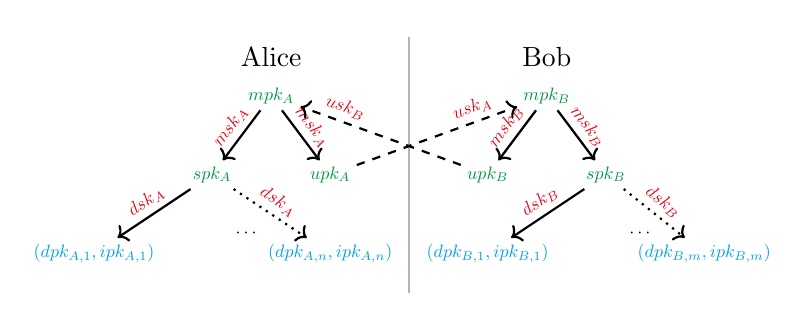
\begin{tikzpicture}
    [
    scale=0.25,
    Separator/.style={-, thick, draw={rgb,255: red,180; green,180; blue,180}},
    Key/.style={draw=none, shape=rectangle,scale=0.65},
    Sign/.style={->, thick,scale=0.65},
    SignKey/.style={midway,sloped,above,scale=0.65},
    CrossSign/.style={->, thick, dashed,scale=0.65},
    DeviceSign/.style={->, thick, dotted,scale=0.65}
    ]

    \node [] (Alice) at (7,  1) {Alice};
    \node [] (Bob)   at (21, 1) {Bob};
    %    \node (Chad) at (52,0) {. };

    \node [] (SeparatorTop)    at (14, 2)   {};
    \node [] (SeparatorBottom) at (14, -11) {};

    \node [style=Key] (AliceMaster)     at (7,    -1) {\sG{$mpk_A$}};
    \node [style=Key] (AliceDevice)     at (4,    -5) {\sG{$spk_A$}};
    \node [style=Key] (AliceUser)       at (10,   -5) {\sG{$upk_A$}};
    \node [style=Key] (AliceDevice1)    at (-2,    -9) {\sB{$(dpk_{A,1}, ipk_{A,1})$}};
    %    \node [style=Key] (AliceDevice2)    at (4,    -9) {$(apk_{A,2}, ipk_{A,2})$};
    \node [style=Key] (AliceDeviceDots) at (5.8,  -8) {$\cdots$};
    \node [style=Key] (AliceDeviceN)    at (10,   -9) {\sB{$(dpk_{A,n}, ipk_{A,n})$}};
    \node [style=Key] (BobMaster)       at (21,   -1) {\sG{$mpk_B$}};
    \node [style=Key] (BobDevice)       at (24,   -5) {\sG{$spk_B$}};
    \node [style=Key] (BobUser)         at (18,   -5) {\sG{$upk_B$}};
    \node [style=Key] (BobDevice1)      at (18,   -9) {\sB{$(dpk_{B,1}, ipk_{B,1})$}};
    %    \node [style=Key] (BobDevice2)      at (23.5,   -9) {$(apk_{B,2}, ipk_{B,2})$};
    \node [style=Key] (BobDeviceDots)   at (25.8, -8) {$\cdots$};
    \node [style=Key] (BobDeviceN)      at (29,   -9) {\sB{$(dpk_{B,m}, ipk_{B,m})$}};

    \draw [style=Separator] (SeparatorTop.center) to (SeparatorBottom.center);

    \draw [style=Sign]       (AliceMaster) -- (AliceDevice)       node            [style=SignKey] {\sR{$msk_A$}};
    \draw [style=Sign]       (AliceMaster) -- (AliceUser)         node            [style=SignKey] {\sR{$msk_A$}};
    \draw [style=Sign] (AliceDevice) -- (AliceDevice1) node [style=SignKey] {\sR{$dsk_A$}};
    %    \draw [style=DeviceSign] (AliceDevice) -- (AliceDevice2) node [style=SignKey] {$dsk_A$};
    \draw [style=DeviceSign] (AliceDevice) -- (AliceDeviceN) node [style=SignKey] {\sR{$dsk_A$}};
    \draw [style=Sign]       (BobMaster)   -- (BobDevice)         node            [style=SignKey] {\sR{$msk_B$}};
    \draw [style=Sign]       (BobMaster)   -- (BobUser)           node            [style=SignKey] {\sR{$msk_B$}};
    \draw [style=Sign] (BobDevice)   -- (BobDevice1)   node [style=SignKey] {\sR{$dsk_B$}};
    %    \draw [style=DeviceSign] (BobDevice)   -- (BobDevice2)   node [style=SignKey] {$dsk_B$};
    \draw [style=DeviceSign] (BobDevice)   -- (BobDeviceN)   node [style=SignKey] {\sR{$dsk_B$}};

    \draw [style=CrossSign] (AliceUser) -- (BobMaster) node [style=SignKey, near end] {\sR{$usk_A$}};
    \draw [style=CrossSign] (BobUser) -- (AliceMaster) node [style=SignKey, near end] {\sR{$usk_B$}};
  \end{tikzpicture}
\end{center}

\end{frame}


\begin{frame}{Device Authentication via Cross-Signing Framework}

\begin{columns}
  \begin{column}{0.5\columnwidth}
  When a new \sB{Device} logs in with account credentials, \sB{Homeserver} allocates a device identifier $D^{A,i}$.

  The \sB{Device} then generates keys for this \sB{Device} and registers it with the \sB{Homeserver}:

  \end{column}
  \begin{column}{0.4\columnwidth}
  \begin{enumerate}
    \item \emph{Long-term Device Keys}, authenticates \textbf{Olm Key Bundle}.
    \item \emph{Olm Key Bundle}, used to establish the pairwise channel, \textbf{Olm}.
  \end{enumerate}
  \end{column}
\end{columns}


\end{frame}

\begin{frame}{Session Establishment via Olm}

\begin{columns}
  \begin{column}{0.5\columnwidth}
    \begin{itemize}
      \small
      \item Bob gets Alice's public key from \sB{Homeserver}
      \item Bob does triple \textbf{D}iffie-\textbf{H}ellman (\textbf{3DH}) to produce a symmetric \textbf{m}aster \textbf{s}ecret.
      \item Bob uses \textbf{Double Ratchet} protocol to derive message keys.
      \item Bob encrypts \textbf{Megolm} \sB{Session State} under these keys, and sends \sB{Session State} to Alice.
    \end{itemize}

  \end{column}
  \begin{column}{0.5\columnwidth}
    \scalebox{0.4}{
      \hspace{-1em}
      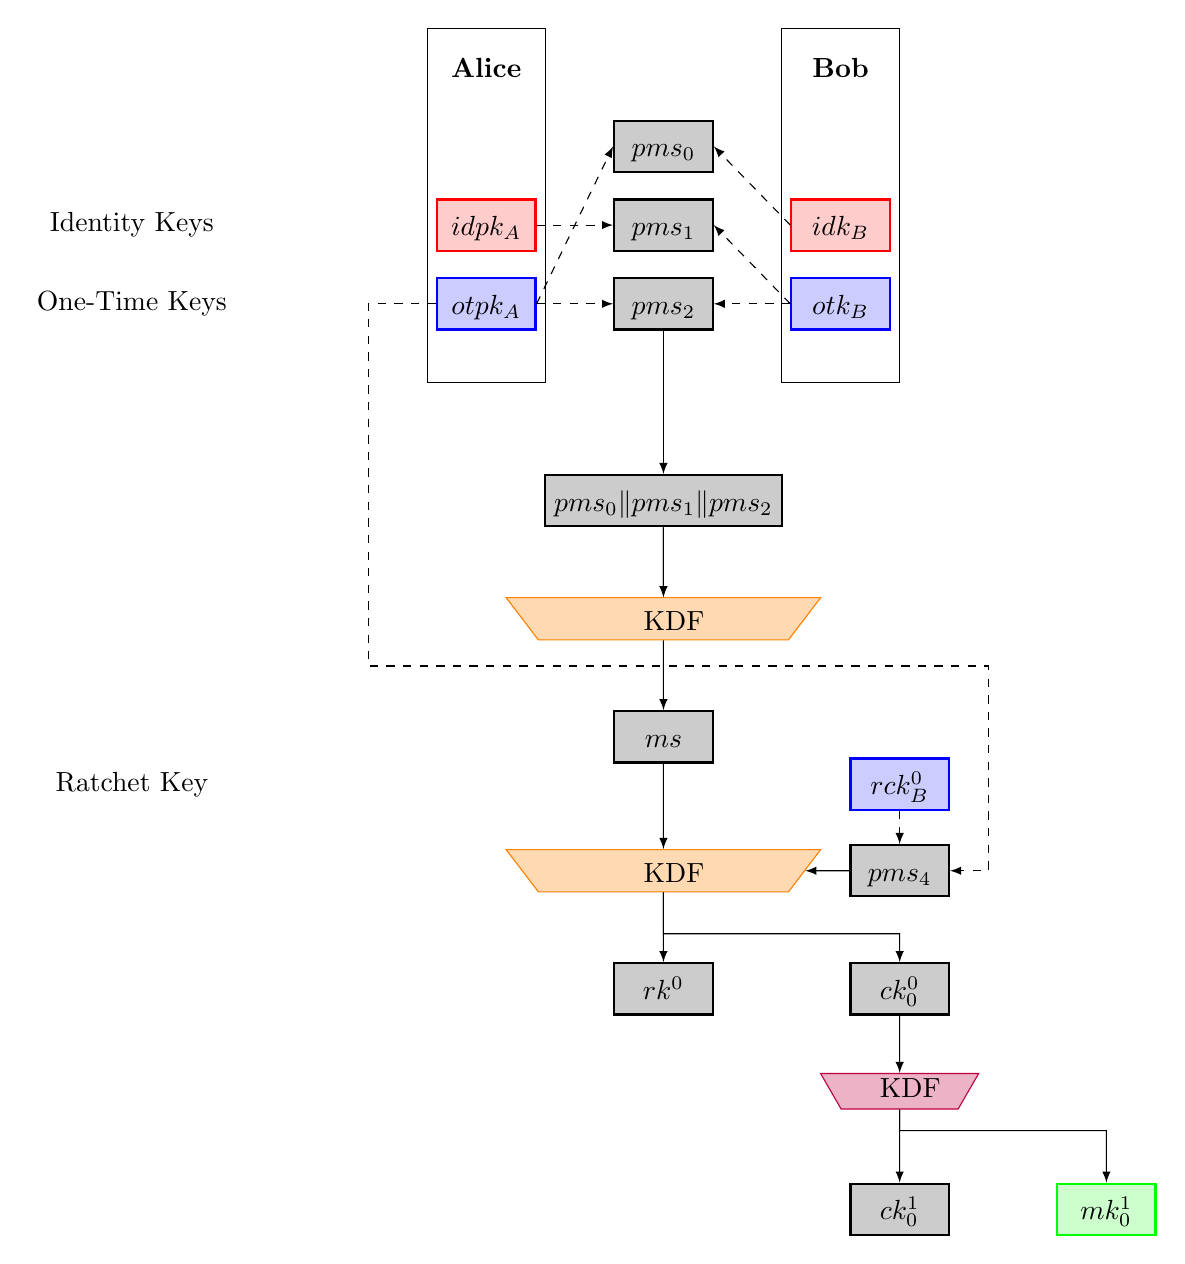
\begin{tikzpicture}[yscale=-2.0,xscale=1.5,>=latex]

        \tikzstyle{keys} = [thick, minimum width=1.25cm, minimum height=0.65cm, text height=2ex, text depth=0.25ex]
        \tikzstyle{identity} = [keys, draw=red, fill=red!20]
        \tikzstyle{reused} = [keys, draw=green, fill=green!20]
        \tikzstyle{ephemeral} = [keys, draw=blue, fill=blue!20]
        \tikzstyle{secret} = [keys, draw=black, fill=black!20]

        \tikzstyle{chainKDF} = [trapezium, minimum width=1.25cm, minimum height=0.45cm, text width=0.5cm, text height=1ex, inner sep=0pt, draw=purple, fill=purple!30, shape border rotate=180]
        \tikzstyle{rootKDF} = [trapezium, minimum width=4cm, text width=0.5cm, text height=2ex, draw=orange, fill=orange!30, shape border rotate=180, trapezium stretches=true, trapezium left angle=80, trapezium right angle=80]
        %\tikzstyle{rootKDF} = [trapezium, minimum width=1.25cm, minimum height=0.45cm, text width=0.5cm, text height=1ex, inner sep=0pt, draw=orange, fill=orange!30, shape border rotate=180]


        % THE HEADINGS

        \node at (0,0) {\textbf{Alice}};
        \node at (3,0) {\textbf{Bob}};
%        \node at (-3,0.5) {Signed Prekey};
        \node at (-3,1)   {Identity Keys};
        \node at (-3,1.5) {One-Time Keys};
        \node at (-3, 4.55) {Ratchet Key};
        \node at (5.25, 6.5) {};

        % BOXES FOR SECRETS

        \draw[-] (-0.5,-0.25) -- (-0.5,2) -- (0.5,2) -- (0.5,-0.25) -- (-0.5, -0.25); %ALICE
        \draw[-] (2.5,-0.25) -- (2.5,2) -- (3.5,2) -- (3.5,-0.25) -- (2.5, -0.25); %BOB

        % SIGNED PREKEY
%        \node[reused] (AlicePreKey) at (0,0.5) {$sppk_A$};

        % IDENTITY KEYS
        \node[identity] (AliceIdKey) at (0,1) {$idpk_A$};
        \node[identity] (BobIdKey) at (3,1) {$idk_B$};

        % ONE TIME KEYS
        \node[ephemeral] (AliceOtKey) at (0,1.5) {$otpk_A$};
        \node[ephemeral] (BobOtKey) at (3,1.5) {$otk_B$};

        % PREMASTER SECRETS

        \node[secret] (pmszero) at (1.5,0.5) {$pms_0$};
        \node[secret] (pmsone) at (1.5,1) {$pms_1$};
        \node[secret] (pmstwo) at (1.5,1.5) {$pms_2$};
%        \node[secret] (pmsthree) at (1.5,2) {$pms_3$};
        \node[secret] (mastersecret) at (1.5,2.75) {$pms_0 \| pms_1\| pms_2$};

        % COMPUTING THE PREMASTER SECRETS

        % PREMASTER SECRET ZEROKDF
        \draw[->,dashed] (BobIdKey.west) -- (pmszero.east);
        \draw[->,dashed] (AliceOtKey.east) -- (pmszero.west);
        % PREMASTER SECRET ONE
        \draw[->,dashed] (BobOtKey.west) -- (pmsone.east);
        \draw[->,dashed] (AliceIdKey.east) -- (pmsone.west);
        % PREMASTER SECRET TWO
        \draw[->,dashed] (BobOtKey.west) -- (pmstwo.east);
        \draw[->,dashed] (AliceOtKey.east) -- (pmstwo.west);
        %PREMASTER SECRET THREE
%        \draw[->,dashed] (BobOtKey.west) -- (pmsthree.east);
%        \draw[->,dashed] (AliceOtKey.east) -- (pmsthree.west);

        % COMPUTING THE MASTER SECRET
        \draw[->] (pmstwo.south) -- (mastersecret.north);

        % COMPUTING THE FIRST ROOT KEY

        \node[rootKDF] (firstrootkdf) at (1.5,3.5) {KDF};
        \draw[->] (mastersecret.south) -- (firstrootkdf.north);
        \node[secret] (rootkeyzero) at (1.5,4.25) {$ms$};
        \draw[->] (mastersecret.south) -- (firstrootkdf.north);
        \draw[->] (firstrootkdf.south) -- (rootkeyzero.north);

        %ALICE'S FIRST RATCHET KEY
        \node[ephemeral] (BobRatKey) at (3.5,4.55) {$rck_{B}^{0}$};

        % COMPUTING THE SECOND ROOT KEY AND FIRST CHAIN KEY

        \node[rootKDF] (secondrootkdf) at (1.5,5.1) {KDF};
        \node[secret] (pmsfour) at (3.5,5.1) {$pms_4$};
        \draw[->, dashed] (AliceOtKey.west) -- (-1,1.5) -- (-1,3.8) -- (4.25,3.8) |- (pmsfour.east);
        \draw[->, dashed] (BobRatKey.south) -- (pmsfour.north);
        \draw[->] (rootkeyzero.south) -- (secondrootkdf.north);
        \draw[->] (pmsfour.west) -- (secondrootkdf.east);
        %FINALLY THE ACTUAL KEYS
        \node[secret] (rootkeyone) at (1.5,5.85) {$rk^{0}$};
        \node[secret] (chainkeyzero) at (3.5,5.85) {$ck^{0}_{0}$};
        \draw[->] (secondrootkdf.south) -- (rootkeyone.north);
        \draw[->] (secondrootkdf.south) -- (1.5,5.5) -| (chainkeyzero.north);

        % EMPTIES
        \node (firstchainkdf) at (3.5,6.5) {};
        \node (chainkeyone) at (3.5,7.25) {};
        \node (messagekeyzero) at (5.25,7.25) {};

        % COMPUTING THE SECOND CHAIN KEY AND THE FIRST MESSAGE KEY
        \node[chainKDF] (firstchainkdf) at (3.5,6.5) {KDF};
        \draw[->] (chainkeyzero.south) -- (firstchainkdf.north);
        \node[secret] (chainkeyone) at (3.5,7.25) {$ck^{1}_{0}$};
        \node[reused] (messagekeyzero) at (5.25,7.25) {$mk^{1}_{0}$};
        \draw[->] (firstchainkdf.south) -- (chainkeyone.north);
        \draw[->] (firstchainkdf.south) -- (3.5,6.75) -| (messagekeyzero.north);

      \end{tikzpicture}
    }

  \end{column}
\end{columns}

\end{frame}

\begin{frame}{Megolm Session}


  \begin{columns}
    \begin{column}{0.53\textwidth}
      \textbf{Megolm} \sB{Session State} allows the \sB{Sender} to encrypt messages to the \textbf{Megolm} channel (resp.~a \sB{Receiver} to decrypt).
    \end{column}
    \begin{column}{0.4\textwidth}
    \scalebox{0.4}{
      \begin{tikzpicture}
        \tikzset{database/.style={
            cylinder,
            aspect=1,
            draw,
            thick,
            fill,
            shape border rotate=90,
            minimum height=4cm,
            left color=black!30,
            right color=black!30,
            middle color=black!30,
            minimum width=5cm,
            path picture={
              \draw[black, thick] let \p1=($(path picture bounding box.north east)-(path picture bounding
              box.south west)$) in
              foreach \XX in {1,2,3}  {([yshift=-\XX*\y1/4]path picture bounding box.north west)
                arc(180:360:\x1/2 and 0.25*\x1/2)};
        }}}

        %% Parties
        \node (MegolmGen) at (-3.5,1) {\LARGE $(gsk,gpk)\gets\SIG.\Gen$};
        \node (MegolmGen) at (-3.5,0) {\LARGE $R\getsr\mathcal{R}$};
        \node (MegolmGen) at (-3.5,-1) {\LARGE $\MegolmIS \gets (0,R,gpk)$};

        \node (AlicePhone) at (0,0)
        {\includegraphics[scale=0.1]{smartphone_diagram.png}};
        \node[alice, minimum size=0.5cm] (Alice) at (-0.5,-0.5) {};

        \node (DavePhone) at (4,0)
        {\includegraphics[scale=0.1]{smartphone_diagram.png}};
        \node[dave, minimum size=0.5cm] (Dave) at (3.5,-0.5) {};

        %% Messages
        \draw[->, ultra thick] (AlicePhone.east)  -- (DavePhone.west) node[midway, above] {\LARGE $\MegolmIS$};

        \node (AP) at (2,-0.4) {\includegraphics[scale=0.02]{signal_icon.png}};
      \end{tikzpicture}
    }
    \end{column}
  \end{columns}

  \vspace{1em}

  A \textbf{Megolm} \sB{session} consists of the current \textit{message index}, the \textit{internal ratchet state}, and the \textit{group signing key}.
  \begin{description}
  \item[\sB{outbound session}] $\MegolmOS = (j, R, \MegolmSK[])$ is kept in the device and used to encrypt messages for the room.
  \item[\sB{inbound session}] $\MegolmIS = (j, R, \MegolmPK[])$ allows other devices in the room to authenticate and decrypt these messages.
  \end{description}

\end{frame}

\begin{frame}{Megolm Ratchet}

  \begin{columns}
    \begin{column}{0.5\columnwidth}
      At its core, \textbf{Megolm } is a symmetric ratcheting scheme:

      \vspace{1em}
      \begin{itemize}
        \item it derives a new key for each message
        \item so that compromise of the current state cannot be used to recover previous encryption state
      \end{itemize}

    \end{column}
    \begin{column}{0.5\columnwidth}
    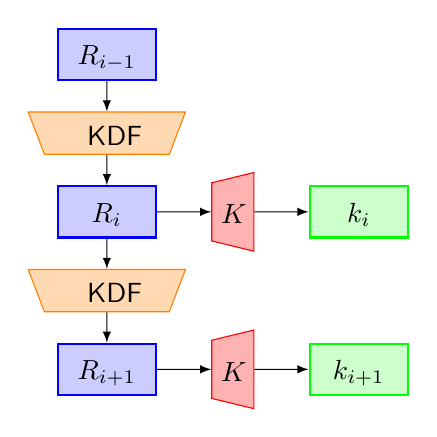
\begin{tikzpicture}[yscale=-1,xscale=0.8,>=latex]
      \tikzstyle{keys} = [thick, minimum width=1.25cm, minimum height=0.65cm, text height=2ex, text depth=0.25ex]
      \tikzstyle{key} = [keys, draw=green, fill=green!20]
      \tikzstyle{random} = [keys, draw=blue, fill=blue!20]
      \tikzstyle{salt} = [keys, draw=black, fill=black!20]
      \tikzstyle{context} = [keys, draw=black, fill=black!20]
      \tikzstyle{KDF} = [trapezium, minimum width=2cm, text width=0.5cm, shape border rotate=180, text height=2ex, draw=orange, fill=orange!30, trapezium stretches=true, trapezium left angle=80, trapezium right angle=80]
      \tikzstyle{roKDF} = [trapezium, minimum width=1cm, text width=0.3cm, shape border rotate=90, text height=2ex, draw=red, fill=red!30, trapezium stretches=true, trapezium left angle=80, trapezium right angle=80]

      \node[random] (KeySource) at (1,0) {$R_{i-1}$};
      \node[KDF] (KDF) at (1,1) {$\KDF$};
      \draw[->] (KeySource.south)  -- (KDF.north);
      \node[random] (ChainZero) at (1,2) {$R_{i}$};
      \node[roKDF] (MsgZero) at (3,2) {$K$};
      \node[key] (KeyOne) at (5,2) {$k_{i}$};
      \draw[->] (ChainZero.east) -- (MsgZero.west);
      \draw[->] (KDF.south) -- (ChainZero.north);
      \node[KDF] (KDFOne) at (1,3) {$\KDF$};
      \draw[->] (ChainZero.south) -- (KDFOne.north);
      \node[random] (ChainOne) at (1,4) {$R_{i+1}$};
      \node[roKDF] (MsgOne) at (3,4) {$K$};
      \draw[->] (KDFOne.south) -- (ChainOne.north);
      \draw[->] (ChainOne.east) -- (MsgOne.west);
      \node[key] (KeyTwo) at (5,4) {$k_{i+1}$};
      \draw[->] (MsgOne.east) -- (KeyTwo.west);
      \draw[->] (MsgZero.east) -- (KeyOne.west);
    \end{tikzpicture}
    \end{column}
  \end{columns}

\end{frame}

\begin{frame}{Advancing the Megolm Ratchet I}

  The interesting part of \textbf{Megolm}: How does the \textbf{Ratchet} advance?
  %  \pause
  %  \begin{center}
    \scalebox{0.8}{
      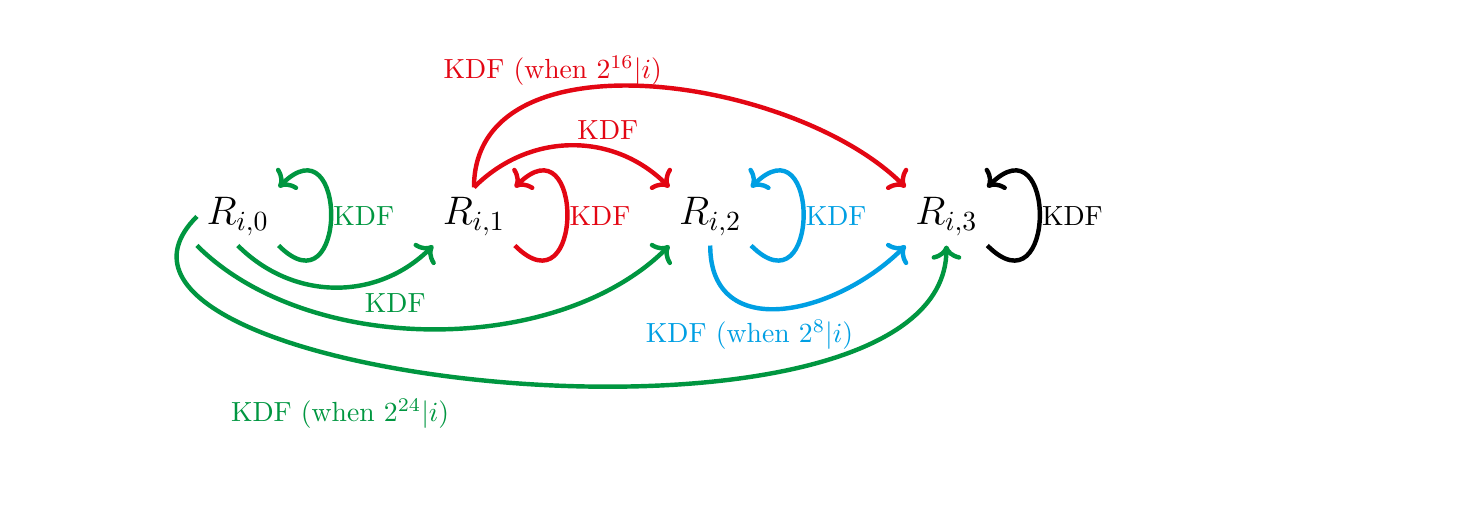
\begin{tikzpicture}
        %% Parties
        \node[] (R0) at (0,0) {\Large $R_{i,0}$};
        \node[] (R1) at (3,0) {\Large $R_{i,1}$};
        \node[] (R2) at (6,0) {\Large $R_{i,2}$};
        \node[] (R3) at (9,0) {\Large $R_{i,3}$};
        \node[] (MT) at (15,0) {\textcolor{white}{a}};

        %% Message
        \pause
        \draw[->, ultra thick] (R3.south east) to[out=-45,in=45,distance=1.25cm] (R3.north east);
        \node[] (R3LBL) at (10.6,0) {KDF};

        \pause
        \draw[->, ultra thick,color=sBlue] (R2.south) to[out=-90,in=225,distance=1.25cm] (R3.south west);
        \draw[->, ultra thick,color=sBlue] (R2.south east) to[out=-45,in=45,distance=1.25cm] (R2.north east);
        \node[] (R2LBL) at (7.6,0) {\sB{KDF}};
        \node[] (R2R3LBL) at (6.5,-1.5) {\sB{KDF (when $2^8|i$)} };

        \pause
        \draw[->, ultra thick,color=sRed] (R1.north) to[out=45,in=135,distance=1cm] (R2.north west);
        \draw[->, ultra thick,color=sRed] (R1.north) to[out=90,in=135,distance=2cm] (R3.north west);
        \draw[->, ultra thick,color=sRed] (R1.south east) to[out=-45,in=45,distance=1.25cm] (R1.north east);
        \node[] (R1LBL) at (4.6,0) {\sR{KDF}};
        \node[] (R1R3LBL) at (4,1.85) {\sR{KDF (when $2^{16}|i$)} };
        \node[] (R1R2LBL) at (4.7,1.1) {\sR{KDF}};


        \pause
        \draw[->, ultra thick,color=sGreen] (R0.south) to[out=-45,in=-135,distance=1cm] (R1.south west);
        \draw[->, ultra thick,color=sGreen] (R0.south west) to[out=-45,in=-135,distance=2cm] (R2.south west);
        \draw[->, ultra thick,color=sGreen] (R0.west) to[out=-135,in=-90,distance=3cm] (R3.south);
        \draw[->, ultra thick,color=sGreen] (R0.south east) to[out=-45,in=45,distance=1.25cm] (R0.north east);
        \node[] (R1LBL) at (1.6,0) {\sG{KDF}};
        \node[] (R1R3LBL) at (1.3,-2.5) {\sG{KDF (when $2^{24}|i$)} };
        \node[] (R1R2LBL) at (2.0,-1.1) {\sG{KDF}};
      \end{tikzpicture}
    }
    %  \end{center}

  Makes catching up after a lot of messages quicker. Since you're constantly copying the ratchet state and advancing, do not need to do $i$ HMAC calls to derive current ratchet state.

\end{frame}

\begin{frame}{Advancing the Megolm Ratchet I}

  We need to advance the \textbf{Megolm} \sB{Ratchet} between encryptions. How?
  \vspace{-0.5cm}
  \begin{multicols}{2}
    \small
    \begin{align*}
      R_{i,0} &=
      \begin{cases}
        \sG{H_0\left(R_{2^{24}(n-1),0}\right)} &\text{if }\exists n | i = 2^{24}n\\
        R_{i-1,0} &\text{otherwise}
      \end{cases}\\
      R_{i,1} &=
      \begin{cases}
        \sG{H_1\left(R_{2^{24}(n-1),0}\right)} &\text{if }\exists n | i = 2^{24}n\\
        \sR{H_1\left(R_{2^{16}(m-1),1}\right)} &\text{if }\exists m | i = 2^{16}m\\
        R_{i-1,1} &\text{otherwise}
      \end{cases}\\
    \end{align*}

    \begin{align*}
      R_{i,2} &=
      \begin{cases}
        \sG{H_2\left(R_{2^{24}(n-1),0}\right)} &\text{if }\exists n | i = 2^{24}n\\
        \sR{H_2\left(R_{2^{16}(m-1),1}\right)} &\text{if }\exists m | i = 2^{16}m\\
        \sB{H_2\left(R_{2^8(p-1),2}\right)} &\text{if }\exists p | i = 2^8p\\
        R_{i-1,2} &\text{otherwise}
      \end{cases}\\
      R_{i,3} &=
      \begin{cases}
        \sG{H_3\left(R_{2^{24}(n-1),0}\right)} &\text{if }\exists n | i = 2^{24}n\\
        \sR{H_3\left(R_{2^{16}(m-1),1}\right)} &\text{if }\exists m | i = 2^{16}m\\
        \sB{H_3\left(R_{2^8(p-1),2}\right)} &\text{if }\exists p | i = 2^8p\\
        H_3\left(R_{i-1,3}\right) &\text{otherwise}
      \end{cases}
    \end{align*}
  \end{multicols}
  \vspace{-0.75cm}
  \begin{align*}
    H_{\sB{i}}(x) &= \hmac(\mathsf{key}=x, \mathsf{input}=\mathtt{0x0\sB{i}})
  \end{align*}

\end{frame}

\begin{frame}{Megolm Encryption}
%  \begin{multicols}{2}

  \begin{enumerate}
    \item \sB{Sender} generates a fresh symmetric key from $R$,
    \item encrypts the message under this key, and
    \item signs it to provide authentication.
  \end{enumerate}

  \begin{center}
  \scalebox{0.5}{
    \begin{tikzpicture}
      \tikzset{database/.style={
          cylinder,
          aspect=1,
          draw,
          thick,
          fill,
          shape border rotate=90,
          minimum height=4cm,
          left color=black!30,
          right color=black!30,
          middle color=black!30,
          minimum width=5cm,
          path picture={
            \draw[black, thick] let \p1=($(path picture bounding box.north east)-(path picture bounding
            box.south west)$) in
            foreach \XX in {1,2,3}  {([yshift=-\XX*\y1/4]path picture bounding box.north west)
              arc(180:360:\x1/2 and 0.25*\x1/2)};
      }}}

      %% LHS Parties
      %        \node[alice, minimum size=1cm] (Alice) at (0,0) {};
      \node[alice, minimum size=1cm] (Bob) at (0,2) {};
%      \node[charlie, minimum size=1cm] (Charlie) at (0,-4) {};


      %% LHS Devices
%      \node (AP) at (4,0) {\includegraphics[scale=0.1]{smartphone_diagram.png}};
      \node (BP) at (4,2) {\includegraphics[scale=0.1]{smartphone_diagram.png}};
%      \node (CP) at (4,4) {\includegraphics[scale=0.1]{smartphone_diagram.png}};

%      \node (CAP) at (4,-4) {\includegraphics[scale=0.1]{smartphone_diagram.png}};

      %% CHANNEL BETWEEN LHS PARTIES AND DEVICES
%      \draw[->, ultra thick] (Bob.east)  -- (AP.west);
      \draw[->, ultra thick] (Bob.east)  -- (BP.west) node[midway, above] {$Enc(k,m)=c$};
%      \draw[->, ultra thick] (Bob.east)  -- (CP.west);

%      \draw[->, ultra thick] (Charlie.east)  -- (CAP.west);

      %% DELIVERY SERVER
      \node[database] (DB1) at (10,2) {};

%      \node[database] (DB2) at (10,-4) {};

      %% CHANNEL BETWEEN HOMESERVERS
%      \draw[<->, ultra thick] ([xshift=0.5cm]DB1.south)  -- ([xshift=0.5cm]DB2.north);
%      \draw[<->, ultra thick] ([xshift=-0.5cm]DB1.south)  -- ([xshift=-0.5cm]DB2.north);

      %% CHANNEL BETWEEN LHS DEVICES AND SERVER
%      \draw[<->, ultra thick] (AP.east)  -- (DB1.west);
      \draw[<->, ultra thick] (BP.east)  -- (DB1.west) node[midway, above] {$c$};
%      \draw[<->, ultra thick] (CP.east)  -- (DB1.west);

%      \draw[<->, ultra thick] (CAP.east)  -- (DB2.west);

      %% RHS Devices
      \node (DP) at (16,0) {\includegraphics[scale=0.1]{smartphone_diagram.png}};
      \node (GP) at (16,2) {\includegraphics[scale=0.1]{smartphone_diagram.png}};
      \node (CBP) at (16,4) {\includegraphics[scale=0.1]{smartphone_diagram.png}};

%      \node (DAP) at (16,-4) {\includegraphics[scale=0.1]{smartphone_diagram.png}};

      %% CHANNEL BETWEEN RHS DEVICES AND SERVER
      \draw[<->, ultra thick] (DB1.east)  -- (DP.west) node[midway, above] {$c$};
      \draw[<->, ultra thick] (DB1.east)  -- (GP.west) node[midway, above] {$c$};
      \draw[<->, ultra thick] (DB1.east)  -- (CBP.west) node[midway, above] {$c$};

%      \draw[<->, ultra thick] (DB2.east)  -- (DAP.west);

      %% RHS Parties
%      \node[bob, minimum size=1cm] (Alice) at (20,2) {};

%      \node[dave, minimum size=1cm] (Dave) at (20,-4) {};

      %% CHANNEL BETWEEN LHS PARTIES AND DEVICES
%      \draw[<->, ultra thick] (DP.east)  -- (Alice.west);
%      \draw[<->, ultra thick] (GP.east)  -- (Alice.west);
%      \draw[<->, ultra thick] (CBP.east)  -- (Alice.west);

%      \draw[<->, ultra thick] (DAP.east)  -- (Dave.west);
    \end{tikzpicture}
  }
\end{center}

    This ciphertext is distributed by the \sB{Homeserver} to other \sB{devices} in the \sB{Group}.

\end{frame}

\begin{frame}{Megolm Decryption}
  \begin{multicols}{2}
    To \sB{decrypt a message}, \sB{Devices} verify the signature with their copy of $\MegolmPK[A,i,G]$, and straightforwardly reverse the process.

    \sB{Receiver Devices} keep the \emph{oldest} copy of the ratchet state, only advancing their ratchet in a temporary copy. This allows \sB{Devices} from the same \sB{User} to share message histories with one another, by sharing old ratchet states.
    \procedureblock{$\mathbf{Megolm.Dec}(\MegolmState, c)$}{
      %
      % Unpack inbound session
      (\MegolmVersion, i, R, \MegolmPK, \MegolmSignature) \assign \MegolmState \\
      %%
      %% Unpack AEAD ciphertext
      (\MegolmVersion', i', c', \tau, \sigma) \assign c \\
      %%
      %% Check signature
      \pcif ! \dsverify(\MegolmPK, \sigma, (\MegolmVersion, i', c', \tau)) \pcthen \\
      \t \pcreturn (\MegolmState, \bot) \\
      %%
      %% Make a copy of the ratchet and advance it to the correct value
      (i, R) \assign \MegolmRatchetAdv^{i'-i}(i, R) \\
      %%
      %% Derive keys from temporary ratchet copy
      k_e \concat k_h \concat k_{iv} \assign \hkdf(0, R', lbl, 80) \\
      %%
      %% Check HMAC
      \pcif \tau \neq \hmac(k_h, (\MegolmVersion, i, c')[0:8] \pcthen \\
      \t  \pcreturn (\MegolmState, \bot) \\
      %%
      %% Decrypt
      m \assign \aescbc.\dec(k_e, k_{iv}, c') \\
      \pcreturn (\MegolmState, m)
    }
\end{multicols}\end{frame}


\begin{frame}{Adding Room Members}

  \begin{itemize}
    \item Alice told by her \sB{Homeserver} that Bob's \sB{Device} has been added.
    \item Alice's \sB{Device} now sends her \textit{current} ratchet state $mgpk = (j,R,gpk)$ to Bob's \sB{Device} using the \textbf{Olm} channel between them
    \item Bob's \sB{Device} can now read messages sent by Alice's \sB{Device} after this point.
  \end{itemize}

  \begin{center}
    \scalebox{0.6}{
      \begin{tikzpicture}
        \tikzset{database/.style={
            cylinder,
            aspect=1,
            draw,
            thick,
            fill,
            shape border rotate=90,
            minimum height=4cm,
            left color=black!30,
            right color=black!30,
            middle color=black!30,
            minimum width=5cm,
            path picture={
              \draw[black, thick] let \p1=($(path picture bounding box.north east)-(path picture bounding
              box.south west)$) in
              foreach \XX in {1,2,3}  {([yshift=-\XX*\y1/4]path picture bounding box.north west)
                arc(180:360:\x1/2 and 0.25*\x1/2)};
        }}}


        %% DELIVERY SERVER
        \node[database] (DB1) at (8,2) {\vspace{-0.25cm} \sB{Homeserver}};

        %% RHS Devices
        \node (AlicePhone) at (16,4)
        {\includegraphics[scale=0.1]{smartphone_diagram.png}};
        \node[alice, minimum size=0.5cm] (Alice) at (15.5,3.5) {};

        \node (BobPhone) at (20,3)
        {\includegraphics[scale=0.2]{smartphone_diagram.png}};
        \node[bob, minimum size=1cm] (Bob) at (19.5,2.5) {};

        %% CHANNEL BETWEEN RHS DEVICES AND SERVER
        \draw[->, ultra thick] (DB1.north east)  -- ([yshift=-0.75cm]AlicePhone.north west) node[midway,above] {\LARGE \textbf{Add} \sB{Bob}};

        \draw[->, ultra thick] (AlicePhone.east)  -- ([yshift=1cm]BobPhone.west) node[midway,above] {\LARGE $mgpk$};
        \node (AP) at (18,3.25) {\includegraphics[scale=0.02]{signal_icon.png}};

        \draw[->, ultra thick] (AlicePhone.south west)  -- ([yshift=1cm]DB1.east) node[midway,below] {\LARGE \textbf{C}};
        \draw[->, ultra thick] ([yshift=-0.75cm]DB1.east)  -- (BobPhone.south west) node[midway,above] {\LARGE \textbf{C}};



      \end{tikzpicture}
    }
  \end{center}
\end{frame}

\begin{frame}{Removing Room Members}

  \begin{itemize}
    \item Alice told by her \sB{homeserver} that Bob's \sB{Device} has been removed.
    \item Alice generates a brand new Megolm ratchet state $mgpk'$
    \item Alice uses her \textbf{Olm} session with all \textit{other} devices in the conversation to send $mgpk'$
    \item Bob's \sB{Device} can no longer read messages sent by Alice's \sB{Device} after this point.
  \end{itemize}

  \begin{center}
    \scalebox{0.5}{
      \begin{tikzpicture}
        \tikzset{database/.style={
            cylinder,
            aspect=1,
            draw,
            thick,
            fill,
            shape border rotate=90,
            minimum height=4cm,
            left color=black!30,
            right color=black!30,
            middle color=black!30,
            minimum width=5cm,
            path picture={
              \draw[black, thick] let \p1=($(path picture bounding box.north east)-(path picture bounding
              box.south west)$) in
              foreach \XX in {1,2,3}  {([yshift=-\XX*\y1/4]path picture bounding box.north west)
                arc(180:360:\x1/2 and 0.25*\x1/2)};
        }}}


        %% DELIVERY SERVER
        \node[database] (DB1) at (8,2) {\vspace{-0.25cm} \sB{Homeserver}};

        %% RHS Devices
        \node (AlicePhone) at (16,4)
        {\includegraphics[scale=0.1]{smartphone_diagram.png}};
        \node[alice, minimum size=0.5cm] (Alice) at (15.5,3.5) {};

        \node (BobPhone) at (20,6)
        {\includegraphics[scale=0.1]{smartphone_diagram.png}};
        \node[bob, minimum size=0.5cm] (Bob) at (19.5,5.5) {};

        \node (CharliePhone) at (20,0)
        {\includegraphics[scale=0.1]{smartphone_diagram.png}};
        \node[charlie, minimum size=0.5cm] (Charlie) at (19.5,-0.5) {};

        %% CHANNEL BETWEEN RHS DEVICES AND SERVER
        \draw[->, ultra thick] (DB1.north east)  -- ([yshift=-0.75cm]AlicePhone.north west) node[midway,above] {\LARGE \textbf{Remove} \sB{Bob}};

        \node (newState) at (16,6) {\LARGE $mgpk' \getsr$};

        \draw[->, ultra thick] (AlicePhone.east)  -- (BobPhone.south west) node[midway,above] {\LARGE $mgpk'$};
        \node (AP) at (18,4) {\includegraphics[scale=0.02]{signal_icon.png}};

        \node (noState) at (18,5) {\Huge \sR{X}};

        \draw[->, ultra thick] (AlicePhone.south east)  -- (CharliePhone.north west) node[midway,above] {\LARGE $~~~~mgpk'$};
        \node (AP) at (18,1.5) {\includegraphics[scale=0.02]{signal_icon.png}};

        \draw[->, ultra thick] (AlicePhone.south west)  -- ([yshift=1cm]DB1.east) node[midway,below] {\LARGE \textbf{C}};
        \draw[->, ultra thick] ([yshift=-0.75cm]DB1.east)  -- (CharliePhone.west) node[midway,above] {\LARGE \textbf{C}};



      \end{tikzpicture}
    }
  \end{center}
\end{frame}


\begin{frame}{``Pursue your dreams but have a backup plan''}

\sB{Backup Functionalities:} \\
\hspace{1em} backup and recover User and Megolm secret values via \sB{Homeservers}.

\vspace{1em}

\begin{columns}
  \begin{column}{0.3\columnwidth}
    \scalebox{0.3}{
      \begin{tikzpicture}
        \tikzset{database/.style={
            cylinder,
            aspect=1,
            draw,
            thick,
            fill,
            shape border rotate=90,
            minimum height=4cm,
            left color=black!30,
            right color=black!30,
            middle color=black!30,
            minimum width=4cm,
            path picture={
              \draw[black, thick] let \p1=($(path picture bounding box.north east)-(path picture bounding
              box.south west)$) in
              foreach \XX in {1,2,3}  {([yshift=-\XX*\y1/4]path picture bounding box.north west)
                arc(180:360:\x1/2 and 0.25*\x1/2)};
            }}}


        %% DELIVERY SERVER
        \node[database] (DB1) at (0,0) {};

        %% RHS Device
        \node (AlicePhoneOne) at (7,2)
        {\includegraphics[scale=0.1]{smartphone_diagram.png}};

        \node (AlicePhoneTwo) at (7,-1)
        {\includegraphics[scale=0.1]{smartphone_diagram.png}};
        \draw[->, ultra thick] (6.5,2)  -- (2,2) node[midway, above] {\LARGE $C$};

        \draw[<-, ultra thick] (6.5,-0.5)  -- (2,-0.5) node[midway, above] {\LARGE $C$};
      \end{tikzpicture}
    }
  \end{column}
  \begin{column}{0.4\columnwidth}
    \scalebox{0.3}{
      \begin{tikzpicture}
        \tikzset{database/.style={
            cylinder,
            aspect=1,
            draw,
            thick,
            fill,
            shape border rotate=90,
            minimum height=4cm,
            left color=black!30,
            right color=black!30,
            middle color=black!30,
            minimum width=5cm,
            path picture={
              \draw[black, thick] let \p1=($(path picture bounding box.north east)-(path picture bounding
              box.south west)$) in
              foreach \XX in {1,2,3}  {([yshift=-\XX*\y1/4]path picture bounding box.north west)
                arc(180:360:\x1/2 and 0.25*\x1/2)};
            }}}


        %% DELIVERY SERVER
        \node[database] (DB1) at (8,2) {};

        %% RHS Devices
        \node (AlicePhone) at (16,4)
        {\includegraphics[scale=0.1]{smartphone_diagram.png}};
        \node[alice, minimum size=0.5cm] (Alice) at (15.5,3.5) {};
        \node (D1) at (16,5.5) {\Large \sB{$D_1$}};

        \node (BobPhone) at (20,3)
        {\includegraphics[scale=0.2]{smartphone_diagram.png}};
        \node[alice, minimum size=1cm] (Bob) at (19.5,2.5) {};
        \node (D2) at (20,5.5) {\Large \sB{$D_2$}};

        %% CHANNEL BETWEEN RHS DEVICES AND SERVER
        % \node (AP) at (11,5.5) {\includegraphics[scale=0.02]{signal_icon.png}};
        \draw[->, ultra thick] (DB1.north east)  |- ([yshift=-0.75cm]AlicePhone.north west) node[midway,above] {\LARGE 1. \textbf{KeyRequest} \sB{$D_2$}};

        \draw[->, ultra thick] (AlicePhone.east)  -- ([yshift=1cm]BobPhone.west) node[midway,above] {\LARGE 2. $mgpk$};
        \node (AP) at (18,5.5) {\includegraphics[scale=0.02]{signal_icon.png}};

        \draw[->, ultra thick] (AlicePhone.south west)  -- ([yshift=1cm]DB1.east) node[midway,below] {\LARGE 3. \textbf{C}};
        \draw[->, ultra thick] ([yshift=-0.75cm]DB1.east)  -- (BobPhone.south west) node[midway,above] {\LARGE 4. \textbf{C}};



      \end{tikzpicture}
    }
  \end{column}
  \begin{column}{0.3\columnwidth}
    \scalebox{0.3}{
      \begin{tikzpicture}
        \tikzset{database/.style={
            cylinder,
            aspect=1,
            draw,
            thick,
            fill,
            shape border rotate=90,
            minimum height=4cm,
            left color=black!30,
            right color=black!30,
            middle color=black!30,
            minimum width=4cm,
            path picture={
              \draw[black, thick] let \p1=($(path picture bounding box.north east)-(path picture bounding
              box.south west)$) in
              foreach \XX in {1,2,3}  {([yshift=-\XX*\y1/4]path picture bounding box.north west)
                arc(180:360:\x1/2 and 0.25*\x1/2)};
            }}}


        %% DELIVERY SERVER
        \node[database] (DB1) at (0,0) {};

        %% RHS Device
        \node (AlicePhoneOne) at (7,2)
        {\includegraphics[scale=0.1]{smartphone_diagram.png}};

        \node (AlicePhoneTwo) at (7,-1)
        {\includegraphics[scale=0.1]{smartphone_diagram.png}};

        \draw[->, ultra thick] (6.5,2)  -- (2,2) node[midway, above] {\LARGE  $(rpk,\sigma)$};

        \draw[<-, ultra thick] (6.5,-0.5)  -- (2,-0.5) node[midway, above] {\LARGE $(rpk,\sigma)$};

        \draw[->, ultra thick] (6.5,-1.5)  -- (2,-1.5) node[midway, below] {\LARGE $(epk,c)$};
      \end{tikzpicture}
    }
  \end{column}
\end{columns}

\vspace{1em}

\begin{columns}[t]
  \begin{column}{0.3\columnwidth}
    \sG{User Secret Backups} \\
    (\textbf{Secure Secret Storage and Sharing (SSSS)})


  \end{column}
  \begin{column}{0.4\columnwidth}
    \sG{Online Session Recovery}\\
    (\textbf{KeyRequest} protocol)

  \end{column}
  \begin{column}{0.3\columnwidth}
    \sG{Offline Session Recovery}\\
    (\textbf{Server-Side Megolm Backups})


  \end{column}
\end{columns}

\begin{columns}[t]
  \begin{column}{0.3\columnwidth}
    \begin{itemize}
    \item backup master (cross-signing) secret keys to server
    \end{itemize}
  \end{column}
  \begin{column}{0.4\columnwidth}
    \begin{itemize}
    \item allows a user's devices to share Megolm session information with each other
    \end{itemize}

  \end{column}
  \begin{column}{0.3\columnwidth}
    \begin{itemize}
    \item as a hybrid of both, backup Megolm sessions to server
    \end{itemize}
  \end{column}
\end{columns}

\end{frame}


\section{Attacks}

\begin{frame}{Q: ``Who to encrypt to?''}
  Group membership is managed through events:

  \centering
  \scalebox{0.75}{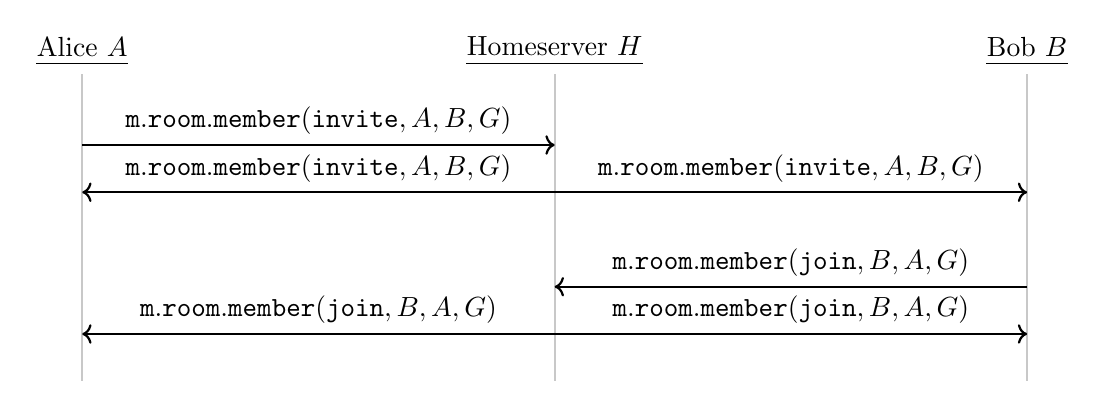
\begin{tikzpicture}
  [
    Actor/.style={shape=rectangle},
    Timeline/.style={-, thick, draw={rgb,255: red,200; green,200; blue,200}},
    ActionLeft/.style={align=right, anchor=south east},
    ActionRight/.style={align=left, anchor=south west},
    MessageArrow/.style={->, thick},
    MessageContents/.style={midway, above, shape=rectangle},
  ]

  \tikzmath{\SeqDiaColumnWidth = 6;};
  \tikzmath{\SeqDiaTextHeight = 0.6;};  % guess
  \tikzmath{\SeqDiaRowHeight = 1.2;};
  \tikzmath{\AliceY = \SeqDiaColumnWidth;};
  \tikzmath{\HomeserverY = 2 * \SeqDiaColumnWidth;};
  \tikzmath{\BobY = 3 * \SeqDiaColumnWidth;};

  % Actor headings
  \node [Actor] at (\AliceY cm, 0 cm) {\uline{Alice $A$}};
  \node [Actor] at (\HomeserverY cm, 0 cm) {\uline{Homeserver $H$}};
  \node [Actor] at (\BobY cm, 0 cm) {\uline{Bob $B$}};

  % Stores the y coordinate of the current row
  \tikzmath{\CurrentY = 0;};

  % Messages
  \tikzmath{\TimelineTop = \CurrentY - 0.5 * \SeqDiaTextHeight;};

  \tikzmath{\CurrentY = \CurrentY-\SeqDiaRowHeight;};
  \draw [MessageArrow] (\AliceY cm, \CurrentY cm) -- (\HomeserverY cm, \CurrentY cm) node [MessageContents] {$\mathtt{m.room.member}(\mathtt{invite}, A, B, G)$};

  % \pause

  \tikzmath{\CurrentY = \CurrentY-\SeqDiaTextHeight;};
  \draw [MessageArrow] (\HomeserverY cm, \CurrentY cm) -- (\AliceY cm, \CurrentY cm) node [MessageContents] {$\mathtt{m.room.member}(\mathtt{invite}, A, B, G)$};
  \draw [MessageArrow] (\HomeserverY cm, \CurrentY cm) -- (\BobY cm, \CurrentY cm) node [MessageContents] {$\mathtt{m.room.member}(\mathtt{invite}, A, B, G)$};

  % \pause

  \tikzmath{\CurrentY = \CurrentY-\SeqDiaRowHeight;};
  \draw [MessageArrow] (\BobY cm, \CurrentY cm) -- (\HomeserverY cm, \CurrentY cm) node [MessageContents] {$\mathtt{m.room.member}(\mathtt{join}, B, A, G)$};

  % \pause

  \tikzmath{\CurrentY = \CurrentY-\SeqDiaTextHeight;};
  \draw [MessageArrow] (\HomeserverY cm, \CurrentY cm) -- (\AliceY cm, \CurrentY cm) node [MessageContents] {$\mathtt{m.room.member}(\mathtt{join}, B, A, G)$};
  \draw [MessageArrow] (\HomeserverY cm, \CurrentY cm) -- (\BobY cm, \CurrentY cm) node [MessageContents] {$\mathtt{m.room.member}(\mathtt{join}, B, A, G)$};

  \tikzmath{\CurrentY = \CurrentY-\SeqDiaTextHeight;};
  \tikzmath{\TimelineBottom = \CurrentY;};

  \begin{pgfonlayer}{background}
      \draw [Timeline] (\AliceY cm,  \TimelineTop cm) -- (\AliceY cm, \TimelineBottom cm);
      \draw [Timeline] (\HomeserverY cm, \TimelineTop cm) -- (\HomeserverY cm, \TimelineBottom cm);
      \draw [Timeline] (\BobY cm, \TimelineTop cm) -- (\BobY cm, \TimelineBottom cm);
  \end{pgfonlayer}
\end{tikzpicture}
}

\end{frame}

\begin{frame}{A: ``Don't worry, the server will let you know.''}
  Group membership is managed through \alert{unauthenticated} events:

  \centering\scalebox{0.75}{\input{unsigned-membership-events-attack-diagram.tikz}}

\end{frame}

\begin{frame}
\frametitle{Discussion}

\begin{columns}[t]
  \begin{column}{0.5\columnwidth}
    \textbf{Matrix knows group administration:}
    \begin{itemize}
    \item Matrix knows of roles and permissions in rooms, including admin roles that control room membership
    \item But there is no cryptographic assurance: encryption, integrity protection, authentication
    \end{itemize}
  \end{column}
  \begin{column}{0.5\columnwidth}
    \textbf{Element offers some ``mitigations'':}
    \begin{itemize}
    \item When a user is added to room this is visible as a genuine membership event
    \item Adding an unverified user to a room, adds a warning to the room that unverified devices are present.
      \begin{itemize}
      \item But just because you verified Alice, does not mean Alice should have access to all your conversations.
      \end{itemize}
    \end{itemize}
  \end{column}
\end{columns}

\end{frame}

\begin{frame}
  \frametitle{Q: ``What are Alice's devices?'' A: ``Don't worry \dots''}

  \begin{itemize}
  \item To send a message to a user, clients need a list of their devices.
    % \pause
  \item This list is \alert{provided by the homeserver} and, hence, can be forged.
  \end{itemize}

\end{frame}

\begin{frame}
  \frametitle{Discussion}
  \begin{columns}[t]
    \begin{column}{0.5\columnwidth}
      \textbf{Matrix has a device verification framework:}
      \begin{itemize}
      \item the list of devices in a room is maintained independently of that
      \item the homeserver may also present different device lists to different users/devices, e.g.~not show the additional malicious device to the user it is purportedly associated with
      \end{itemize}
    \end{column}
    \begin{column}{0.5\columnwidth}
      \textbf{Element does offer a ``mitigation'':}
      \begin{itemize}
      \item adding an unverified device to a room will lead to a warning that such a device is present
      \end{itemize}
    \end{column}
  \end{columns}
\end{frame}

\begin{frame}
  \frametitle{Damage}
  Breaks confidentiality: \emph{Attackers can eavesdrop on conversations }
  \vspace{1em}
  with \emph{some} indication in (Element's) user interface.
\end{frame}

\begin{frame}
  \frametitle{Status}
  Neither of these two are fixed, but a remediation (signed group membership messages) is in the planning stage.
  \begin{itemize}
  \item Matrix' previous rational: Element client shows list of users for a room, so users can inspect, i.e.~burden on users.
  \item Matrix post-disclosure: ``many in the cryptography community consider this a serious misdesign. Eitherway, it’s avoidable behaviour and we’re ramping up work now to address it by signing room memberships so the clients control membership rather than the server.''
  \end{itemize}
\end{frame}

\begin{frame}{Attack on Out-of-Band Verification}
  \scalebox{0.6}{
    \begin{tikzpicture}[overlay]

      %% Parties
      \node (AlicePhone) at (16,-5)
      {\includegraphics[scale=0.1]{smartphone_diagram.png}};
      \node[alice, minimum size=0.5cm] (Alice) at (15.5,-5.5) {};

      \node (CharliePhone) at (22,-5)
      {\includegraphics[scale=0.1]{smartphone_diagram.png}};
      \node[charlie, minimum size=0.5cm] (Charlie) at (21.5,-5.5) {};

      \draw[->, ultra thick] (AlicePhone.east)  -- (CharliePhone.west) node[midway, above] {\includegraphics[scale=0.4]{emoji-verif.png}};
    \end{tikzpicture}
  }

  How to ensure connection is not being MITM-ed? Out-of-band verification! \\
  \vspace{0.5em}
  Short Authentication String (SAS) protocol $\approx$
  \begin{enumerate}
    \item Key exchange to generate a shared secret.
    \item Compare the shared secret out-of-band\\ \hspace{2em} \alert{(using short strings of emojis)}.
    \\ If they don't match, abort!
    \item Send correct cryptographic identities to each other over a secure channel (constructed using the shared secret).
  \end{enumerate}
  % \pause

  \alert{The homeserver tricks devices into sharing a homeserver-controlled identity.}

\end{frame}

\begin{frame}{Attack on Out-of-Band Verification}
\begin{columns}[t]
  \begin{column}{0.5\columnwidth}
  \begin{itemize}
  \item Two types of verification:
    \begin{enumerate}
    \item Between two users
    \item Between two devices of the same user
    \end{enumerate}
  \item Each party sends the other a message containing a ``key identifier'' field:
    \begin{enumerate}
    \item For two users, this field contains the fingerprint of their \alert{master cross-signing key}, $\MasterPK$.
    \item For two devices, this field contains their \alert{device identifier}.
    \end{enumerate}
  \end{itemize}

  \end{column}
  \begin{column}{0.5\columnwidth}
\textbf{Attack:}
\begin{itemize}
\item Homeserver assigns the target a \alert{device identifier} that is also a \alert{master cross-signing key} fingerprint \emph{that the homeserver generated}.
\item When the target sends a verification request message with their device identifier, the receiving device interprets it as a cross-signing key fingerprint and signs it!
\end{itemize}

  \end{column}
\end{columns}

\end{frame}

\begin{frame}[fragile]
  \frametitle{The Spec}

  \begin{columns}
    \begin{column}{0.4\columnwidth}
      \textbf{Out-of-band verification is used for:}
      \begin{enumerate}
      \item two users' devices verify each other; and,
      \item a user verifies a new device.
      \end{enumerate}

   \end{column}
    \begin{column}{0.6\columnwidth}

      \textit{``Verification methods can be used to verify a user’s master key by using the master public key, encoded using unpadded base64, as the device ID, and treating it as a normal device. For example, if Alice and Bob verify each other using SAS, Alice’s m.key.verification.mac message to Bob may include ``ed25519:alices+master+public+key'': ``alices+master+public+key'' in the mac property. Servers therefore must ensure that device IDs will not collide with cross-signing public keys.''}

  \end{column}
\end{columns}

\framebreak{}

\end{frame}

\begin{frame}[fragile]
  \frametitle{Message Format}

  \begin{minted}[fontsize=\footnotesize]{js}
{"mac": {"ed25519:<mpk'>": SAS.CalcMAC(k, dpk, c || "ed25519:<mpk'>"),
         "ed25519:<mpk>":  SAS.CalcMAC(k, mpk, c || "ed25519:<mpk>"),},
 "keys": SAS.CalcMAC(k, sort("ed25519:<mpk'>", "ed25519:<mpk>"), c || "KEY_IDS")}
  \end{minted}

    An \MsgTypeVerificationMAC{} message generated by a user with cross-signing master verification key $\MasterPK$, long-term device key $\DevicePK$ and device identifier $\MasterPK$' (which is also the master verification key of a homeserver controlled cross-signing identity).
    Whilst the two entries in the \texttt{mac} dictionary could be distinguished by the differing second argument given to $\SASCalculateMAC$, $\SASVerifyMAC$ interprets the first entry as a device, and then passes it to $\SASSignMAC$ which interprets it as a cross-signing identity.

\end{frame}

\begin{frame}[allowframebreaks]
  \frametitle{Attack}

  Alice $A$ and Bob $B$, each with device $D_{A,1}$ and $D_{B,1}$ respectively. Additionally, they are both registered to a malicious homeserver, whose aim is to compromise their out-of-band verification with the SAS protocol. The attack proceeds as follows:
  \begin{enumerate}
  \item When Alice $A$ registers their account with the homeserver, the homeserver generates a parallel cross-signing identity with verification keys $(\MasterPK[A]', \SelfPK[A]', \UserPK[A]')$.
  \item When Alice $A$ logs in for the first time, the homeserver sets the device identifier $D_{A,1} \assign \MasterPK[A]'$.
  \item When Bob $B$ logs in for the first time, the homeserver sets $D_{B,1}$ as normal.
  \item Alice and Bob each setup their own cross-signing identities with verification keys $(\MasterPK[A], \SelfPK[A], \UserPK[A])$ and $(\MasterPK[B], \SelfPK[B], \UserPK[B])$ respectively. They upload these to the homeserver.
   \framebreak
  \item The homeserver proceeds to present two versions of the cross-signing state:
    \begin{enumerate}
    \item When Alice requests their own cross-signing information, they are presented with the version they uploaded $(\MasterPK[A], \SelfPK[A], \UserPK[A])$.
    \item When Bob requests Alice's cross-signing information, they are presented with the version generated by the malicious homeserver $(\MasterPK[A]', \SelfPK[A]', \UserPK[A]')$.
    \end{enumerate}
  \framebreak
  \item Alice and Bob perform an out-of-band verification using the SAS protocol. At the end, they exchange \MsgTypeVerificationMAC{} messages containing their cryptographic identity (for signing).
    \(D_{B,1}\) processes it as follows:
    \begin{enumerate}
    \item $\SASVerifyMAC$ interprets the entry for $\MasterPK[A]'$ as a request for device verification. It fetches the expected device identity key $\DevicePK[A,1]$, then calculates a matching MAC. The device identity key pulled from the homeserver is legitimate, and matches the one used by Alice's device to generate the MAC\@. Thus, the message passes verification.
    \item $\SASSignMAC$ interprets the entry for $\MasterPK[A]'$ as a request for cross-signing verification. This is because the homeserver has led Bob's client to believe that Alice's cross-signing identity is $\MasterPK[A]'$.
    \end{enumerate}
  \item Bob cross-signs the homeserver controlled identity for Alice, and uploads the signature to the homeserver to distribute to their other devices.
  \end{enumerate}

\end{frame}

\begin{frame}
  \frametitle{Damage}
  Breaks confidentiality: \emph{Attackers can eavesdrop on conversations} \\
  \vspace{1em}
  \hspace{1em} and authentication: \emph{Attackers can impersonate users} \\
  \vspace{1em}
  with \alert{no indication} in (Element's) user interface!
\end{frame}

\begin{frame}
  \frametitle{Take Home Message}

  \centering
  \includegraphics[height=1.0\textheight]{./all-the-things.jpg}

\end{frame}

\begin{frame}{Alice: \dots, Bob: ``Here are the keys for Charley'', Alice: ``Ta!''}
  When a user adds a new device, they'd like that device to be able to decrypt messages previously sent to that user via the \textbf{KeyRequest} protocol.

  Element and other clients limited who they sent secrets \alert{to} \\
  but not who they accepted secrets \alert{from}.

  \textbf{Attack:}

  \centering\scalebox{0.75}{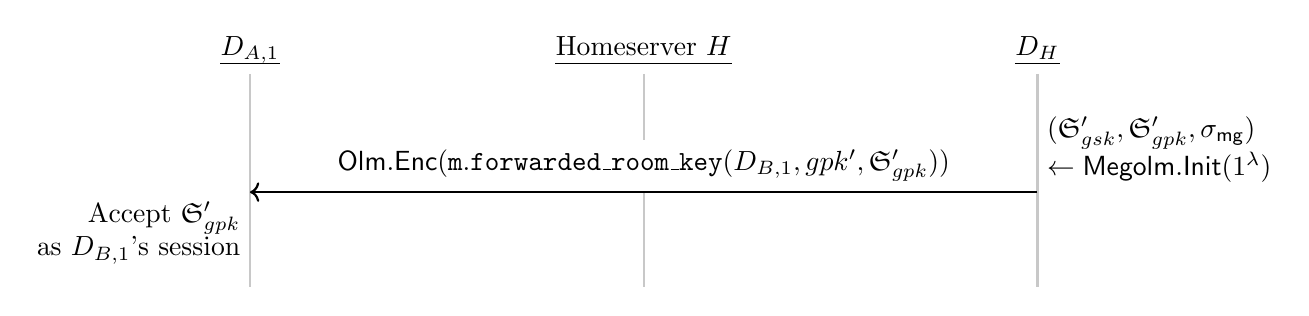
\begin{tikzpicture}
  [
    Actor/.style={shape=rectangle},
    Timeline/.style={-, thick, draw={rgb,255: red,200; green,200; blue,200}},
    ActionLeft/.style={align=right, anchor=south east},
    ActionRight/.style={align=left, anchor=south west},
    MessageArrow/.style={->, thick},
    MessageContents/.style={midway, above, shape=rectangle},
  ]

  \tikzmath{\SeqDiaColumnWidth = 5;};
  \tikzmath{\SeqDiaTextHeight = 0.6;};  % guess
  \tikzmath{\SeqDiaRowHeight = 1.2;};
  \tikzmath{\AliceOneY = \SeqDiaColumnWidth;};
  \tikzmath{\HomeserverY = 2 * \SeqDiaColumnWidth;};
  \tikzmath{\AliceTwoY = 3 * \SeqDiaColumnWidth;};

  % Actor headings
  \node [Actor] at (\AliceOneY cm, 0 cm) {\uline{$D_{A,1}$}};
  \node [Actor] at (\HomeserverY cm, 0 cm) {\uline{\alert{Homeserver $H$}}};
  \node [Actor] at (\AliceTwoY cm, 0 cm) {\uline{\alert{$D_{H}$}}};

  % Stores the y coordinate of the current row
  \tikzmath{\CurrentY = 0;};

  % Messages
  \tikzmath{\TimelineTop = \CurrentY - 0.5 * \SeqDiaTextHeight;};

  \tikzmath{\CurrentY = \CurrentY-\SeqDiaTextHeight;};
  \tikzmath{\CurrentY = \CurrentY-\SeqDiaRowHeight;};

  \node [ActionRight, anchor=south west] at (\AliceTwoY cm, \CurrentY cm) {$(\MegolmOS', \MegolmIS', \MegolmSignature)$ \\ $\assign \MegolmInit(\secparam)$};

  \draw [MessageArrow] (\AliceTwoY cm, \CurrentY cm) -- (\AliceOneY cm, \CurrentY cm)
    node [MessageContents, fill=white] {$\OlmEnc(\MsgTypeFwdRoomKey(D_{B,1}, gpk', \MegolmIS'))$};
  \node [ActionLeft, anchor=north east] at (\AliceOneY cm, \CurrentY cm) {\alert{Accept $\MegolmIS'$} \\ \alert{as $D_{B,1}$'s session}};

  \tikzmath{\CurrentY = \CurrentY-\SeqDiaRowHeight;};
  \tikzmath{\TimelineBottom = \CurrentY;};

  \begin{pgfonlayer}{background}
      \draw [Timeline] (\AliceOneY cm,  \TimelineTop cm) -- (\AliceOneY cm, \TimelineBottom cm);
      \draw [Timeline] (\HomeserverY cm, \TimelineTop cm) -- (\HomeserverY cm, \TimelineBottom cm);
      \draw [Timeline] (\AliceTwoY cm, \TimelineTop cm) -- (\AliceTwoY cm, \TimelineBottom cm);
  \end{pgfonlayer}
\end{tikzpicture}
}

\end{frame}


\begin{frame}
  \frametitle{Damage}
  \begin{columns}[t]
  \begin{column}{0.3\columnwidth}
    \textbf{Semi-trusted Impersonation Attack}\\
    \vspace{1em}
    Breaks authentication: \emph{Attackers can impersonate users} \\
    \vspace{1em}
    with some indication in (Element's) user interface.
  \end{column}
  \begin{column}{0.3\columnwidth}
  \end{column}
  \begin{column}{0.3\columnwidth}
  \end{column}
  \end{columns}

\end{frame}

\begin{frame}{Layering Attacks for Full Impersonation}
  Megolm session setup:

  \begin{center}
  \scalebox{0.5}{
    \renewcommand{\pause}{} % hack (we want to skip the \pause's within the below figure)
    \begin{tikzpicture}
      \tikzset{database/.style={
          cylinder,
          aspect=1,
          draw,
          thick,
          fill,
          shape border rotate=90,
          minimum height=4cm,
          left color=black!30,
          right color=black!30,
          middle color=black!30,
          minimum width=5cm,
          path picture={
            \draw[black, thick] let \p1=($(path picture bounding box.north east)-(path picture bounding
            box.south west)$) in
            foreach \XX in {1,2,3}  {([yshift=-\XX*\y1/4]path picture bounding box.north west)
              arc(180:360:\x1/2 and 0.25*\x1/2)};
      }}}

      %% Parties
      \node (AlicePhone) at (0,0)
      {\includegraphics[scale=0.1]{smartphone_diagram.png}};
      \node[alice, minimum size=0.5cm] (Alice) at (-0.5,-0.5) {};

      \node (BobPhone) at (11,2)
      {\includegraphics[scale=0.1]{smartphone_diagram.png}};
      \node[bob, minimum size=0.5cm] (Bob) at (10.5,1.5) {};

      \node (CharliePhone) at (11,0)
      {\includegraphics[scale=0.1]{smartphone_diagram.png}};
      \node[charlie, minimum size=0.5cm] (Charlie) at (10.5,-0.5) {};


      \node (MegolmGenOne) at (-3,2) {\LARGE $\MegolmInit$};
      \node (MegolmGenTwo) at (-3,0) {\LARGE $(\MegolmOS,\MegolmIS,\MegolmSignature)$};
      \draw[->] (MegolmGenOne.south) -- (MegolmGenTwo.north);

      % \pause

      %% Messages
      \draw[->, ultra thick] (AlicePhone.north)  |- (BobPhone.west) node[midway, above right] {\LARGE $c_0 = \OlmEnc(k_{AB},(\MegolmIS,\MegolmSignature))$};

      % \pause
      %        \draw[->, ultra thick] (AlicePhone.south)  |- (DavePhone.west) node[midway, below right] {\LARGE $c_2 = \Olm.\Encrypt(k_{AD},\MegolmIS)$};
      \draw[->, ultra thick] (AlicePhone.east)  -- (CharliePhone.west) node[midway, above] {\LARGE $c_1 = \OlmEnc(k_{AC},(\MegolmIS,\MegolmSignature))$};
    \end{tikzpicture}
  }
  \end{center}

  What if we could send $(\MegolmIS, \MegolmSignature)$ over Megolm instead of Olm?

  Could we send it over a Megolm session placed via previous impersonation attack?

\end{frame}

\begin{frame}{Layering Attacks for Full Impersonation}
  Device $D_{H}$ impersonates $D_{B,1}$ to $D_{A,1}$:

  \centering\scalebox{0.75}{\input{trusted-impersonation-attack-diagram.tikz}}

\end{frame}

\begin{frame}
  \frametitle{Damage}
  \begin{columns}
  \begin{column}{0.3\columnwidth}
    \textbf{Semi-trusted Impersonation Attack}\\
    \vspace{1em}
    Breaks authentication: \emph{Attackers can impersonate users} \\
    \vspace{1em}
    with some indication in (Element's) user interface.
  \end{column}
  \begin{column}{0.3\columnwidth}
    \textbf{Fully-trusted Impersonation Attack}\\
    \vspace{1em}
    Breaks authentication: \emph{Attackers can impersonate users} \\
    \vspace{1em}
    with \alert{no indication} in (Element's) user interface.
  \end{column}
  \begin{column}{0.3\columnwidth}
  \end{column}
  \end{columns}
\end{frame}

\begin{frame}{More Layers: Authentication to Confidentiality Break}
  When a user verifies their new device, it will use \textbf{SSSS} to request \sB{User Secrets} from the user's existing devices.

  This includes the \textbf{recovery key} used for \textbf{Megolm Backups}, i.e.

  \centering\scalebox{0.75}{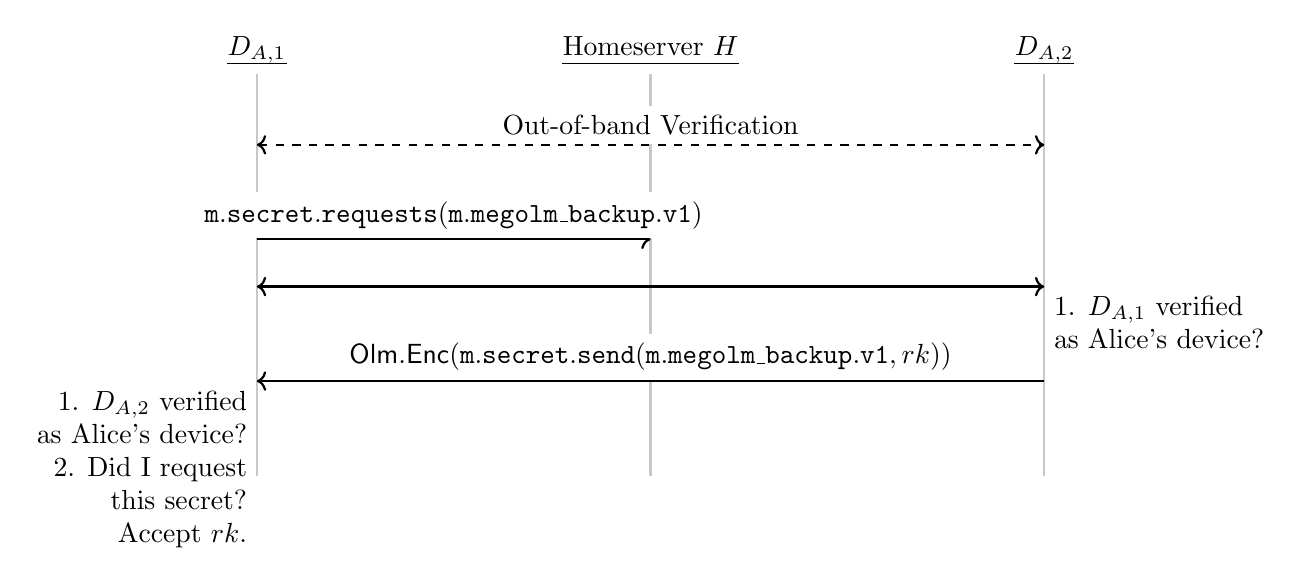
\begin{tikzpicture}
  [
    Actor/.style={shape=rectangle},
    Timeline/.style={-, thick, draw={rgb,255: red,200; green,200; blue,200}},
    ActionLeft/.style={align=right, anchor=south east},
    ActionRight/.style={align=left, anchor=south west},
    MessageArrow/.style={->, thick},
    MessageContents/.style={midway, above, shape=rectangle},
	SubprotocolArrow/.style={<->, thick, dashed},
	SubprotocolContents/.style={midway, above, shape=rectangle}
  ]

  \tikzmath{\SeqDiaColumnWidth = 5;};
  \tikzmath{\SeqDiaTextHeight = 0.6;};  % guess
  \tikzmath{\SeqDiaRowHeight = 1.2;};
  \tikzmath{\AliceOneY = \SeqDiaColumnWidth;};
  \tikzmath{\HomeserverY = 2 * \SeqDiaColumnWidth;};
  \tikzmath{\AliceTwoY = 3 * \SeqDiaColumnWidth;};

  % Actor headings
  \node [Actor] at (\AliceOneY cm, 0 cm) {\uline{$D_{A,1}$}};
  \node [Actor] at (\HomeserverY cm, 0 cm) {\uline{Homeserver $H$}};
  \node [Actor] at (\AliceTwoY cm, 0 cm) {\uline{$D_{A,2}$}};

  % Stores the y coordinate of the current row
  \tikzmath{\CurrentY = 0;};

  % Messages

  \tikzmath{\TimelineTop = \CurrentY - 0.5 * \SeqDiaTextHeight;};

  \tikzmath{\CurrentY = \CurrentY-\SeqDiaRowHeight;};
  \draw [SubprotocolArrow] (\AliceOneY cm, \CurrentY cm) -- (\AliceTwoY cm, \CurrentY cm)
    node [SubprotocolContents, fill=white] {Out-of-band Verification};

  % \pause

  \tikzmath{\CurrentY = \CurrentY-\SeqDiaRowHeight;};
  \draw [MessageArrow] (\AliceOneY cm, \CurrentY cm) -- (\HomeserverY cm, \CurrentY cm)
    node [MessageContents, fill=white] {$\MsgTypeSecretsRequest(\mathtt{m.megolm\_backup.v1})$};

  \tikzmath{\CurrentY = \CurrentY-\SeqDiaTextHeight;};
  \draw [MessageArrow] (\HomeserverY cm, \CurrentY cm) -- (\AliceOneY cm, \CurrentY cm)
    node [MessageContents] {};
  \draw [MessageArrow] (\HomeserverY cm, \CurrentY cm) -- (\AliceTwoY cm, \CurrentY cm)
    node [MessageContents] {};
  \node [ActionRight, anchor=north west] at (\AliceTwoY cm, \CurrentY cm) {1. $D_{A,1}$ verified \\ as Alice's device?};

  % \pause

  \tikzmath{\CurrentY = \CurrentY-\SeqDiaRowHeight;};

  \draw [MessageArrow] (\AliceTwoY cm, \CurrentY cm) -- (\AliceOneY cm, \CurrentY cm)
    node [MessageContents, fill=white] {$\OlmEnc(\MsgTypeSecretsSend(\mathtt{m.megolm\_backup.v1}, rk))$};
  \node [ActionLeft, anchor=north east] at (\AliceOneY cm, \CurrentY cm)
    {1. $D_{A,2}$ verified \\ as Alice's device? \\ 2. Did I request \\ this secret? \\ Accept $rk$.};

  \tikzmath{\CurrentY = \CurrentY-\SeqDiaRowHeight;};
  \tikzmath{\TimelineBottom = \CurrentY;};

  \begin{pgfonlayer}{background}
      \draw [Timeline] (\AliceOneY cm,  \TimelineTop cm) -- (\AliceOneY cm, \TimelineBottom cm);
      \draw [Timeline] (\HomeserverY cm, \TimelineTop cm) -- (\HomeserverY cm, \TimelineBottom cm);
      \draw [Timeline] (\AliceTwoY cm, \TimelineTop cm) -- (\AliceTwoY cm, \TimelineBottom cm);
  \end{pgfonlayer}
\end{tikzpicture}
}

\end{frame}

\begin{frame}
  \frametitle{Damage}
  \begin{columns}
  \begin{column}{0.3\columnwidth}
    \textbf{Semi-trusted Impersonation Attack}\\
    \vspace{1em}
    Breaks authentication: \emph{Attackers can impersonate users} \\
    \vspace{1em}
    with some indication in (Element's) user interface.
  \end{column}
  \begin{column}{0.3\columnwidth}
    \textbf{Fully-trusted Impersonation Attack}\\
    \vspace{1em}
    Breaks authentication: \emph{Attackers can impersonate users} \\
    \vspace{1em}
    with \alert{no indication} in (Element's) user interface.
  \end{column}
  \begin{column}{0.3\columnwidth}
    \textbf{Authentication to Confidentiality Break}\\
    \vspace{1em}
    Breaks confidentiality: \emph{Attackers can eavesdrop on conversations} \\
    \vspace{1em}
    with \alert{no indication} in (Element's) user interface.
  \end{column}
  \end{columns}

  \vspace{2em}

  \centering
    {\large Together: \emph{complete break of confidentiality and authentication!}}

\end{frame}

\begin{frame}
  \frametitle{Take Home Messages}


  \begin{itemize}
  \item There is no confidentiality without authentication.
  \item Put all cryptographic code in one small core.\footnote{Element checked authentication at \emph{display} time, rather than at receipt time and thus those checks were not run for messages that are not displayed.}
  \end{itemize}
\end{frame}

\begin{frame}
  \frametitle{IND-CCA Vulnerability}

  \begin{itemize}
  \item Matrix uses an encrypt-then-MAC encryption scheme composing \(\aesctr\) with \(\hmacsha256\).
  \item Recall that \(\aesctr\) proceeds by encrypting a series of blocks \(iv, iv \oplus 1, iv \oplus 2, \ldots\) and XORing the result onto the message blocks \(m_{i}\) to produce the ciphertext blocks \(c_{i}\).
  \item The full ciphertext is \(iv \| c_{0} \| c_{1} \| \ldots \). However, the \(iv\) is not covered by the authentication tag produced by \(\hmacsha256\).
  \end{itemize}

\end{frame}

\begin{frame}
  \frametitle{IND-CCA Attack}

Let \(c*\) be some challenge ciphertext for either some message \(m_{0}\) or \(m_{1}\) of length 128 bits:
\[
  c* \coloneqq iv \| \aes(k_0, iv) \oplus m_b \| \hmac(k_1, \aes(k_0, iv) \oplus m_b).
\]
The adversary requests an encryption of zero from the encryption oracle and receives
\[
  c \coloneqq  iv' \| \aes(k_0,iv') \oplus 0 \| \hmac\big(k_1, \aes(k_0,iv') \oplus 0\big)
\]
for some \(iv'\). Finally, the adversary requests a decryption of
\[
  c^+ \coloneqq  iv \|  \aes({k_0, iv'}) \oplus 0 \| \hmac\big(k_1, \aes(k_0,iv') \oplus 0\big)
\]
from the decryption oracle. Note that the MAC verifies correctly, and so the adversary will receive \(`t \coloneqq \aes(k_0, iv') \oplus \aes(k_0, iv) \oplus 0\). Given that the adversary already knows \(\aes(k_0, iv')\) it can now recover \(\aes(k_0,iv) = t \oplus \aes(k_0, iv')\) and thus decrypt the challenge \(c*\).
\end{frame}

\begin{frame}{IND-CCA Attack Limitations}
  \begin{columns}[t]
    \begin{column}{0.5\columnwidth}
      \begin{itemize}
      \item Forwarding keys to the target and observing the resulting backups on the homeserver provides an encryption oracle.

      \item Modifying a backup on the homeserver then requesting the resulting key provides a decryption oracle.
      \end{itemize}
    \end{column}
    \begin{column}{0.5\columnwidth}

      \begin{itemize}
      \item In Matrix, \(k_{0}, k_{1}\) are bound to a particular \(\MegolmPK\) and all secret \(R\)'s associated with a \(\MegolmPK\) can be obtained by the key request protocol.
      \item Any modified ciphertexts will likely be invalid JSON structures and fail to parse correctly (preventing the decryption oracle from sharing the plaintext with the adversary).
      \end{itemize}
    \end{column}
  \end{columns}
\end{frame}

\begin{frame}
  \frametitle{Attachments}

  \begin{itemize}
  \item A similar issue exists for attachments which are shared out of band in encrypted form.
  \item Here the hash shared over Megolm (which takes the role of the MAC) does not include the \(iv\)\@.
  \item Since the \(iv\) itself is also shared over Megolm and thus implicitly authenticated, we do not see a way to exploit this behaviour.
  \end{itemize}
\end{frame}

\begin{frame}
  \frametitle{Take home message:}

  There is no confidentiality without integrity.\footnote{Corollary: The CIA triad -- confidentiality, integrity, availability -- is nonsense.}

\end{frame}


\begin{frame}
  \frametitle{Recap \& Status}
  \begin{enumerate}
  \item \alert{Trivial confidentiality breaks} not yet fixed
  \item \alert{Attack on out-of-band verification} \href{https://nvd.nist.gov/vuln/detail/CVE-2022-39250}{CVE-2022-39250}; reportedly mitigated
  \item \alert{Impersonation}  \href{https://nvd.nist.gov/vuln/detail/CVE-2022-39246}{CVE-2022-39246},
\href{https://nvd.nist.gov/vuln/detail/CVE-2022-39249}{CVE-2022-39249} and
\href{https://nvd.nist.gov/vuln/detail/CVE-2022-39257}{CVE-2022-39257};\footnote{In their review of the ecosystem the Matrix developers discovered further clients vulnerable to variants of our attack and assigned
\href{https://nvd.nist.gov/vuln/detail/CVE-2022-39252}{CVE-2022-39252},
\href{https://nvd.nist.gov/vuln/detail/CVE-2022-39254}{CVE-2022-39254} and
\href{https://nvd.nist.gov/vuln/detail/CVE-2022-39264}{CVE-2022-39264}.} reportedly mitigated
  \item \alert{Full impersonation} \href{https://nvd.nist.gov/vuln/detail/CVE-2022-39248}{CVE-2022-39248},
\href{https://nvd.nist.gov/vuln/detail/CVE-2022-39251}{CVE-2022-39251} and \href{https://nvd.nist.gov/vuln/detail/CVE-2022-39255}{CVE-2022-39255}; reportedly mitigated
  \item \alert{Impersonation to confidentiality break} same CVEs as above; reportedly mitigated
  \item \alert{Theoretical confidentiality attack} not yet fixed
  \end{enumerate}
\end{frame}

\section{Discussion}

\begin{frame}{Difficult Problems!}
  Matrix aims to solve some difficult problems:
  \begin{enumerate}
    \item Secure (Group) Messaging \\
    \dots in a multi-device setting, \\
    \dots that is scalable to thousands of devices in a single group.
    \item Backups and history sharing.
    \item Authentication and identity verification \\
    \dots cross-signing to reduce user burden of out-of-band verification.
    \item Federation.
    \item Supporting a variety of clients across many platforms.
  \end{enumerate}

\end{frame}



\begin{frame}{Cryptography is not a dark art}


  \begin{tabular}[t]{@{}cp{0.5\textwidth}}
    \adjustbox{valign=t}{\includegraphics[width=0.25\textwidth]{drake-top.jpg}} &
    ``Crypto is hard!''
    \only<2>{ \newline Of course, cryptography is hard, so is any other science.}\\
    \adjustbox{valign=t}{\includegraphics[width=0.25\textwidth]{drake-bottom.jpg}} &
    \only<3>{ Modern cryptography gives us the tools to reason about cryptographic protocols to rule out the sort of issues we found here. }
    \only<4>{``Cryptography needs security models and proofs!''}
  \end{tabular}
\end{frame}

\begin{frame}{Cryptography is not a dark art}
  \begin{tikzpicture}[remember picture, overlay]
    \node[] at (current page.center) {
      \fbox{\includegraphics[width=0.5\textwidth]{thomas.png}}
    };
  \end{tikzpicture}
\end{frame}

\section{Getting started on knocking stuff over}

\begin{frame}
  \frametitle{Two approaches}

  \begin{columns}
    \begin{column}{0.5\columnwidth}
      \textbf{Start from the attack}
      \begin{itemize}
      \item Start from a vulnerability (e.g.~IV reuse)
      \item Think about where the relevant primitive is used
      \item Search for protocols until you find one that is broken
      \end{itemize}
    \end{column}
    \begin{column}{0.5\columnwidth}
      \textbf{Start from a protocol/scheme}
      \begin{itemize}
      \item Start from a protocol you care about
      \item Read spec/source code
      \item Identify cryptographic core, focus on that
      \item Need to have a good idea what is out there in terms of attacks
      \end{itemize}
    \end{column}
\end{columns}

\end{frame}

\begin{frame}
  \frametitle{Cryptographic proof attempts are cryptanalysis}

  \begin{itemize}
  \item Our project started with the intention to prove Matrix secure (see Ben's talk)
  \item We obviously could not make the proof work.
  \item Eventually the attacks became so many that we decided to write an ``attack paper'' first
  \end{itemize}

  Try to prove more protocols out there secure! If you fail, you get an attack paper, if you succeed you get a proof paper!
\end{frame}

\begin{frame}
  \frametitle{Disclosure lessons}
  \begin{itemize}
  \item Decide who you have a responsibility to.
    \begin{itemize}
    \item This does not have to include the developers, the security state or even the main users.
    \end{itemize}
  \item Typically you will attack a protocol/scheme/product developed by people with no rigorous security or cryptography training.
    \begin{itemize}
    \item They may plead, threaten, bribe.
    \item You can educate them, but you do not owe them this.
    \end{itemize}
  \item Usually things sour when you move towards public disclosure
    \begin{description}
    \item[Developer incentive] minimise perception of impact
    \item[Your incentive] maximise perception of impact
    \end{description}
  \item Security Twitter will be on your side with silly takes, don't join in, don't ridicule, but educate
  \end{itemize}
\end{frame}

\begin{frame}[standout]{Fin}
  \begin{center}
    \Huge Thank you! Questions?
  \end{center}
  \url{https://nebuchadnezzar-megolm.github.io/}
\end{frame}

\end{document}


%%% Local Variables:
%%% mode: latex
%%% TeX-master: t
%%% TeX-engine: xetex
%%% TeX-command-extra-options: "-shell-escape"
%%% End:
